\documentclass[../DefinizioneDiProdotto.tex]{subfiles}
\begin{document}
		\section{Specifica delle componenti}
			\subsection{SWEDesigner}
				I package contenuti al suo interno sono:
				\begin{itemize}
					\item SWEDesigner::Client;
					\item SWEDesigner::Server.
				\end{itemize}
				Questo package non contiene delle classi.
			\subsection{SWEDesigner::Client}
				% IMMAGINE ARCHITETTURA CLIENT GENERALE
				\begin{figure}[H]\label{fig:ClientSubsystem}
					\centering
					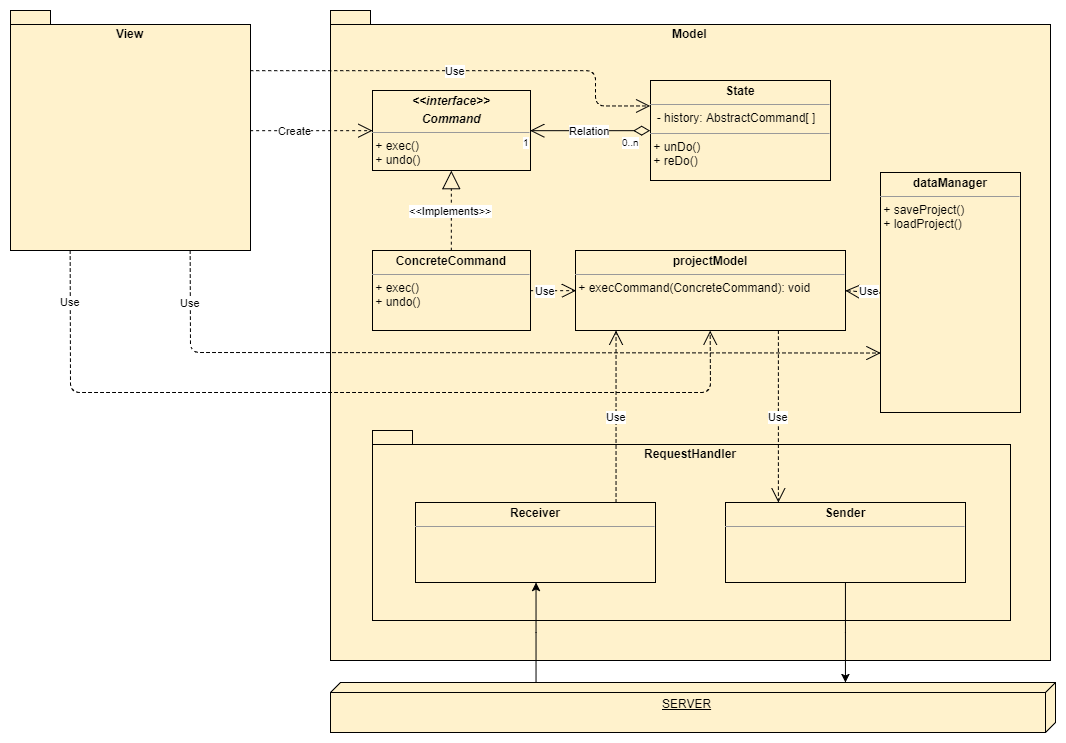
\includegraphics[scale=0.46]{Immagini/DiagrammaArchitettura/ClientSubsystem.png}
					\caption{Architettura del client}
				\end{figure}
				I package contenuti al suo interno sono:
				\begin{itemize}
					\item SWEDesigner::Client::Model;
					\item SWEDesigner::Client::View.
				\end{itemize}
				Questo package non contiene delle classi.
			\subsection{SWEDesigner::Client::Model}
				\hypertarget{SWEDesigner::Client::Model}
				I package contenuti al suo interno sono:
				\begin{itemize}
					\item SWEDesigner::Client::Model::Items.
				\end{itemize}
				Le classi contenute al suo interno verranno elencate qui di seguito.

				\subsubsection{SWEDesigner::Client::Model::DataManager}
				\hypertarget{SWEDesigner::Client::Model::DataManager}{}
					\begin{itemize}
						\item \textbf{Tipo}: \emph{Classe statica};
						\item \textbf{Descrizione}: Si occupa della persistenza dei dati, in particolare del salvataggio su file system locale del progetto già esistente.\\;
						\item \textbf{Metodi}:
						\begin{itemize}
							\item \emph{newProject(): void} \\
							Dopo aver chiesto conferma all'utente, crea un nuovo progetto sovrascrivendo quello correntemente aperto; \\
							\item \emph{openProject(): void} \\
							Legge un file JSON e ne salva il contenuto in project e nel projectModel come progetto attualmente aperto; \\
							\item \emph{save(fileName: String): void} \\
							Salva i dati del progetto, li converte in formato JSON e avvia la procedura di download in locale del browser; \\
							\textbf{Parametri}:
							\begin{itemize}
								\item \emph{fileName: String}
								Nome del file generato da scaricare; \\
							\end{itemize}
							\item \emph{saveAs(): void}\\
							Estrae la stringa inserita dall'utente nella schermata per il salvataggio con nome e invoca la il metodo per il salvataggio del progetto corrente in un file con il nome desiderato; \\
						\end{itemize}
						\item \textbf{Relazioni con le altre classi}:
						\begin{itemize}
							\item OUT \hyperlink{SWEDesigner::Client::Model::ProjectModel}{\emph{SWEDesigner::Client::Model::ProjectModel}}: si occupa di gestire la parte logica dell'editor;
							\item OUT \hyperlink{SWEDesigner::Client::Model::Project}{\emph{SWEDesigner::Client::Model::Project}}: si occupa di gestire gli elementi contenuti nel diagramma.
						\end{itemize}
					\end{itemize}

				\subsubsection{SWEDesigner::Client::Model::ProjectModel}
				\hypertarget{SWEDesigner::Client::Model::ProjectModel}{}
					% IMMAGINE ARCHITETTURA MAINMODEL
					\begin{figure}[H]\label{fig:Model}
						\centering
						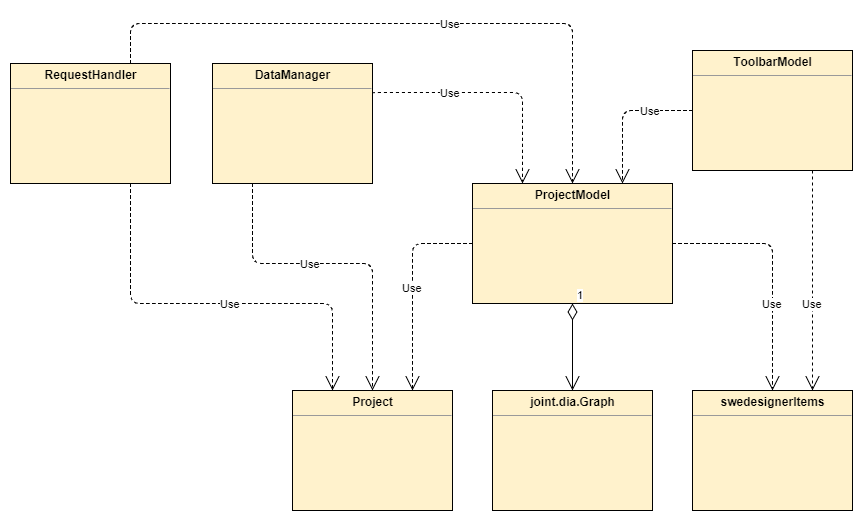
\includegraphics[scale=0.46]{Immagini/DiagrammaArchitettura/MainModel.png}
						\caption{Architettura di Model}
					\end{figure}

					\begin{itemize}
						\item \textbf{Tipo}: \emph{Classe};
						\item \textbf{Descrizione}: Model del progetto corrente. Si occupa di gestire il graph (joint.dia.Graph) e tutti gli eventi ad esso associati;
						\item \textbf{Padre}: \emph{Backbone.model};
						\item \textbf{Attributi}:
						\begin{itemize}
							\item \emph{currentDiagram: String} \\
							L'id del diagramma correntemente caricato nel graph (null se è il diagramma dei package); \\
							\item \emph{currentDiagramType: String} \\
							Il tipo del diagramma correntemente caricato nel graph ("packageDiagram", "classDiagram" o "bubbleDiagram"); \\
							\item \emph{graph: joint.dia.Graph} \\
							Il model dell'area di disegno associata al paper della \hyperlink{SWEDesigner::Client::View::ProjectView}{\emph{SWEDesigner::Client::View::ProjectView}}; \\
							\item \emph{itemToBeAdded: String} \\
							Salvataggio temporaneo dell'elemento da aggiungere al graph corrente; \\
						\end{itemize}
						\item \textbf{Metodi}:
						\begin{itemize}
							\item \emph{addItem(item: Object): void} \\
							Salva in itemToBeAdded l'elemento passato in input che è un oggetto di Swedesigner::Client::Model::Items; \\
								\textbf{Parametri}:
								\begin{itemize}
									\item \emph{item: Object}
									Elemento del diagramma; \\
								\end{itemize}
							\item \emph{addItemToGraph(): void} \\
							Aggiunge un elemento al grafo del diagramma corrente; \\
							\item \emph{changedPosition(graph: joint.dia.Graph, cell: joint.dia.Cell, newPosition: Object, opt: Object): void} \\
							Gestisce la traslazione di un elemento selezionato nel grafo; \\
								\textbf{Parametri}:
								\begin{itemize}
									\item \emph{graph: joint.dia.Graph}
									Grafo del diagramma corrente; \\
									\item \emph{cell: joint.dia.Cell}
									Elemento correntemente selezionato; \\
									\item \emph{newPosition: Object}
									Posizione attuale dell'oggetto nel grafo; \\
									\item \emph{opt: Object}
									Traslazione dell'oggetto dalla posizione iniziale alla posizione "newPosition"; \\
								\end{itemize}
							\item \emph{deleteCell(): void} \\
							Rimuove un elemento dal grafo eliminando anche gli eventuali diagrammi derivati (classi o bubble); \\
							\item \emph{deleteOperation(): void} \\
							Rimuove un'operazione ed eventualmente anche il diagramma delle bubble associato; \\
							\item \emph{getCellFromId(cellId: String): void} \\
							Ritorna l'elemento del graph avente l'id passato come parametro in input; \\
								\textbf{Parametri}:
								\begin{itemize}
									\item \emph{cellId: String}
									Identificativo dell'elemento nel graph; \\
								\end{itemize}
							\item \emph{graphSwitched(): void} \\
							Genera l'evento "switchgraph"; \\
							\item \emph{initialize(): void} \\
							Inizializzazione del ProjectModel: inizializzazione del graph, del currentDiagramType, degli eventi verificabili; \\
							\item \emph{resizeParent(parent: Object): void} \\
							Esegue il resize di un elemento del diagramma ingrandendolo; \\
								\textbf{Parametri}:
								\begin{itemize}
									\item \emph{parent: Object}
									Elemento del diagramma; \\
								\end{itemize}
							\item \emph{saveCurrentDiagram(): void} \\
							Salva il diagramma correntemente aperto all'interno della struttura definita nella classe Project; \\
							\item \emph{switchInGraph(): void} \\
							Esegue lo switch in profondità al diagramma selezionato svuotando il graph dagli elementi correntemente presenti e caricando gli eventuali nuovi elementi; \\
							\item \emph{switchOutGraph(): void} \\
							Esegue lo switch all'antistante tipo di diagramma selezionato svuotando il graph dagli elementi correntemente presenti e caricando gli eventuali nuovi elementi; \\
						\end{itemize}
						\item \textbf{Relazioni con le altre classi}:
						\begin{itemize}
							\item IN \hyperlink{SWEDesigner::Client::Model::DataManager}{\emph{SWEDesigner::Client::Model::DataManager}}: si occupa della persistenza dei dati, in particolare del salvataggio su file system locale del progetto e del caricamento di un progetto già esistente;
							\hyperlink{SWEDesigner::Client::Model::ToolbarModel}{\emph{SWEDesigner::Client::Model::ToolbarModel}}: È il componente del programma che si occupa di gestire la parte logica della toolbar;
							\item IN \hyperlink{SWEDesigner::Client::Model::RequestHandler}{\emph{SWEDesigner::Client::Model::RequestHandler}}: si occupa di gestire i dati ricevuti dal server;
							\item OUT \hyperlink{SWEDesigner::Client::Model::Project}{\emph{SWEDesigner::Client::Model::Project}}: si occupa di gestire gli elementi contenuti nel diagramma;
							\item OUT \hyperlink{SWEDesigner::Client::Model::Items::Swedesigner}{\emph{SWEDesigner::Client::Model::Items::Swedesigner}}: è il contenitore degli elementi che si possono inserire in un diagramma.
						\end{itemize}
					\end{itemize}

				\subsubsection{SWEDesigner::Client::Model::ToolbarModel}
				\hypertarget{SWEDesigner::Client::Model::ToolbarModel}{}
					\begin{itemize}
						\item \textbf{Tipo}: \emph{Classe};
						\item \textbf{Descrizione}: È il componente del programma che si occupa di gestire la parte logica della toolbar;
						\item \textbf{Padre}: \emph{Backbone.model};
						\item \textbf{Attributi}:
						\begin{itemize}
							\item \emph{items: Object} \\
							Contiene tutti gli elementi definibili nel diagramma corrente; \\
						\end{itemize}
						\item \textbf{Metodi}:
						\begin{itemize}
							\item \emph{addElement(id: String): void} \\
							Salva lo strumento selezionato interagendo con il \hyperlink{SWEDesigner::Client::Model::ProjectModel}{\emph{SWEDesigner::Client::Model::ProjectModel}}; \\
							\textbf{Parametri}:
							\begin{itemize}
								\item \emph{id: String}
								Identificativo del tipo di strumento/elemento da inserire; \\
							\end{itemize}
							\item \emph{createItems(): void} \\
							Assegna al campo dati "items" il set di strumenti utilizzabili nel diagramma corrente; \\
							\item \emph{currentDiagram(): String} \\
							Ritorna il tipo del diagramma corrente; \\
							\item \emph{initialize(): void} \\
							Inizializzazione del ToolbarModel: chiama il metodo createItems;
						\end{itemize}
						\item \textbf{Relazioni con le altre classi}:
						\begin{itemize}
							\item OUT \hyperlink{SWEDesigner::Client::Model::ProjectModel}{\emph{SWEDesigner::Client::Model::ProjectModel}}: si occupa di gestire la parte logica dell'editor;
							\item OUT \hyperlink{SWEDesigner::Client::Model::Items::Swedesigner}{\emph{SWEDesigner::Client::Model::Items::Swedesigner}}: è il contenitore degli elementi che si possono inserire in un diagramma.
						\end{itemize}
					\end{itemize}

				\subsubsection{SWEDesigner::Client::Model::Project}
				\hypertarget{SWEDesigner::Client::Model::Project}{}
					\begin{itemize}
						\item \textbf{Tipo}: \emph{Classe};
						\item \textbf{Descrizione}: Contenitore di tutti gli elementi del progetto correntemente aperto nella Single Page Application;
						\item \textbf{Padre}: \emph{Backbone.model};
						\item \textbf{Attributi}:
						\begin{itemize}
							\item \emph{classes: Object} \\
							Contiene: classesArray (array contentente diagrammi delle classi; in ogni indice è presente un oggetto {id: idPackagePadre, items: [arrayClassiDelDiagramma]}) e dependenciesArray (array contenente i link del corrispondente diagramma delle classi; in ogni indice è presente un oggetto {id: idPackagePadre, items: [arrayLinkDelDiagramma]}); \\
							\item \emph{operations: Array<Object>} \\
							Contiene un array di oggetti; in ogni indice è presente un oggetto {id: id dell'operazione, items: [arrayBubbleDelDiagramma]}); \\
							\item \emph{packages: Object} \\
							Contiene: packagesArray (array contenente i package item del diagramma dei package) e dependenciesArray (array contenente i link del diagramma dei package); \\
						\end{itemize}
						\item \textbf{Metodi}:
						\begin{itemize}
							\item \emph{deleteClassesDiagramOfPkg(id: String): void} \\
							Elimina il diagramma delle classi associato al package e tutti i diagrammi delle bubble associati alle operazioni delle relative classi; \\
							\textbf{Parametri}:
							\begin{itemize}
								\item \emph{id: String}
								Identificativo del package; \\
							\end{itemize}
							\item \emph{deleteOperationDiagram(id: String): void} \\
							Elimina il diagramma delle bubble associato all'operazione; \\
							\textbf{Parametri}:
							\begin{itemize}
								\item \emph{id: String}
								Identificativo dell'operazione; \\
							\end{itemize}
							\item \emph{getClassIndex(id: String): Number} \\
							Cerca ed eventualmente ritorna l'indice dell'array classesArray del diagramma delle classi associato al package; \\
							\textbf{Parametri}:
							\begin{itemize}
								\item \emph{id: String}
								Identificativo del package; \\
							\end{itemize}
							\item \emph{getOperationIndex(id: String): Number} \\
							Cerca ed eventualmente ritorna l'indice dell'array operations del diagramma delle bubble associato all'operazione; \\
							\textbf{Parametri}:
							\begin{itemize}
								\item \emph{id: String}
								Identificativo dell'operazione; \\
							\end{itemize}
						\end{itemize}
						\item \textbf{Relazioni con le altre classi}:
						\begin{itemize}
							\item IN \hyperlink{SWEDesigner::Client::Model::ProjectModel}{\emph{SWEDesigner::Client::Model::ProjectModel}}: si occupa di gestire la parte logica dell'editor;
							\item IN \hyperlink{SWEDesigner::Client::Model::DataManager}{\emph{SWEDesigner::Client::Model::DataManager}}: si occupa della persistenza dei dati, in particolare del salvataggio su file system locale del progetto e del caricamento di un progetto già esistente;
							\item IN \hyperlink{SWEDesigner::Client::Model::RequestHandler}{\emph{SWEDesigner::Client::Model::RequestHandler}}: si occupa di gestire i dati ricevuti dal server;
						\end{itemize}
					\end{itemize}
				
				\subsubsection{SWEDesigner::Client::Model::RequestHandler}
				\hypertarget{SWEDesigner::Client::Model::RequestHandler}{}
					\begin{itemize}
						\item \textbf{Tipo}: \emph{Classe};
						\item \textbf{Descrizione}: Si occupa della gestione delle comunicazioni tra client e server (lato client);
						\item \textbf{Padre}: \emph{Backbone.model};
						\item \textbf{Metodi}:
						\begin{itemize}
							\item \emph{caricaJa(): void} \\
							Carica il file json nel server e ne genera il codice Java restituendo il nome della cartella compressa; \\
							\item \emph{caricaJs(): void} \\
							Carica il file json nel server e ne genera il codice Javascript restituendo il nome della cartella compressa; \\
						\end{itemize}
						\item \textbf{Relazioni con le altre classi}:
						\begin{itemize}
							\item OUT \hyperlink{SWEDesigner::Client::Model::ProjectModel}{\emph{SWEDesigner::Client::Model::ProjectModel}}: si occupa di gestire la parte logica dell'editor;
							\item OUT \hyperlink{SWEDesigner::Client::Model::Project}{\emph{SWEDesigner::Client::Model::Project}}: si occupa di gestire gli elementi contenuti nel diagramma.
						\end{itemize}
					\end{itemize}
		
			%inizio parte Giulio
			
			\subsection{SWEDesigner::Client::Model::Items}
			\hypertarget{SWEDesigner::Client::Model::Items}{}
			Questo package non contiene dei sottopackage. Le classi contenute al suo interno verranno
			elencate qui di seguito.
			
			\subsubsection{SWEDesigner::Client::Model::Items::Swedesigner}
			\hypertarget{SWEDesigner::Client::Model::Items::Swedesigner}{}
			\begin{itemize}
				\item \textbf{Tipo}: \emph{Class};
				\item \textbf{Descrizione}: Collezione di oggetti che si possono inserire all'interno di un diagramma suddivisi per tipo di diagramma;
				\item \textbf{Relazioni con le altre classi}:
				\begin{itemize}
					\item IN SWEDesigner::Client::Model::ProjectModel
					\item IN SWEDesigner::Client::Model::toolbarModel
				\end{itemize}
			\end{itemize}
			
			%--------------------------------------PACKAGE DIAGRAM--------------------------------------
			
			\subsubsection[Swedesigner.model.packageDiagram.items.Base]{SWEDesigner::Client::Model::Items::\\Swedesigner.model.packageDiagram.items.Base}
			\hypertarget{SWEDesigner::Client::Model::Items::Swedesigner.model.packageDiagram.items.Base}{}
			\begin{itemize}
				\item \textbf{Tipo}: \emph{Class};
				\item \textbf{Descrizione}: Elemento base generico per diagramma dei package UML;
				\item \textbf{Padre}: \emph{joint.shapes.basic.Generic};
				\item \textbf{Attributi}:
				\begin{itemize}
					\item \emph{toolMarkup: string}\\
					Markup HTML per la rappresentazione grafica;
					\item \emph{defaults: Object}\\
					Attributi di default per l'oggetto;
				\end{itemize}
				\item \textbf{Metodi}:
				\begin{itemize}
					\item \emph{initialize(): void}\\
					Inizializzazione di Base: imposta evento al verificarsi del cambio dei valori e chiama il metodo per la renderizzazione dell'item;
					\item \emph{updateRectangles(): void}\\
					Render dell'item;
					\item \emph{getValues(): Object}\\
					Ritorna i valori dell'item;
					\item \emph{setToValue(value: Object, path: string): void}\\
					Imposta "values.path" a "value";
					Parametri:
					\begin{itemize}
						\item \emph{value: Object} \\
						Valore da assegnare;
						\item \emph{path: string} \\
						Percorso al membro;
					\end{itemize}
				\end{itemize}
			\end{itemize}
			
			
			\subsubsection[Swedesigner.model.packageDiagram.items.BaseView]{SWEDesigner::Client::Model::Items::\\Swedesigner.model.packageDiagram.items.BaseView}
			\hypertarget{SWEDesigner::Client::Model::Items::Swedesigner.model.packageDiagram.items.BaseView}{}
			\begin{itemize}
				\item \textbf{Tipo}: \emph{Class};
				\item \textbf{Descrizione}: View per item "Base";
				\item \textbf{Padre}: \emph{joint.dia.ElementView};
				\item \textbf{Metodi}:
				\begin{itemize}
					\item \emph{initialize(): void}\\
					Inizializzazione di BaseView: chiama il metodo "initialize" della classe "Base" e imposta un evento alla reazione del model chiamando sequenzialmente i metodi "update" e "resize";
					\item \emph{render(): Object}\\
					Render dell'item;
					\item \emph{renderTools(): Object}\\
					Assistenza al metodo "render" per la renderizzazione dell'item;
				\end{itemize}
			\end{itemize}
			
			\subsubsection[Swedesigner.model.packageDiagram.items.Package]{SWEDesigner::Client::Model::Items::\\Swedesigner.model.packageDiagram.items.Package}
			\hypertarget{SWEDesigner::Client::Model::Items::Swedesigner.model.packageDiagram.items.Package}{}
			\begin{itemize}
				\item \textbf{Tipo}: \emph{Class};
				\item \textbf{Descrizione}: Elemento package per diagramma dei package UML;
				\item \textbf{Padre}: \emph{Swedesigner.model.packageDiagram.items.Base};
				\item \textbf{Attributi}:
				\begin{itemize}
					\item \emph{markup: string}\\
					Markup HTML per la rappresentazione grafica;
					\item \emph{defaults: Objects}\\
					Attributi di default per l'oggetto Package (tipo, posizione, dimensione, attributi CSS, stato e contenuto dell'oggetto);
				\end{itemize}
				\item \textbf{Metodi}:
				\begin{itemize}
					\item \emph{initialize(): void}\\
					Inizializzazione di Package: chiama il metodo "initialize" della classe base e crea l'istanza di Diagram associata al diagramma delle classi relativo al package;
					\item \emph{getPackageName(): string}\\
					Ritorna il nome del Package;
					\item \emph{updateRectangles(): void}\\
					Render del package;
				\end{itemize}
			\end{itemize}
			
			\subsubsection[Swedesigner.model.packageDiagram.items.PkgComment]{SWEDesigner::Client::Model::Items::\\Swedesigner.model.packageDiagram.items.PkgComment}
			\hypertarget{SWEDesigner::Client::Model::Items::Swedesigner.model.packageDiagram.items.PkgComment}{}
			\begin{itemize}
				\item \textbf{Tipo}: \emph{Class};
				\item \textbf{Descrizione}: Commento per diagramma dei package UML;
				\item \textbf{Padre}: \emph{joint.shapes.basic.TextBlock};
				\item \textbf{Attributi}:
				\begin{itemize}
					\item \emph{toolMarkup: string}\\ 
					Markup HTML per la rappresentazione grafica;
					\item \emph{defaults: Objects}\\
					Attributi di default per l'oggetto PkgComment;
				\end{itemize}
				\item \textbf{Metodi}:
				\begin{itemize}
					\item \emph{initialize(): void}\\
					Inizializzazione di PkgComment;
					\item \emph{getPackageName(): string}\\
					Ritorna il nome del Package;
					\item \emph{getValues(): Objects}\\
					Ritorna i valori dell'item PkgComment;
					\item \emph{setToValue(value: Object, path: string): void}\\
					Imposta "values.path" a "value";
					Parametri:
					\begin{itemize}
						\item \emph{value: Object} \\
						Valore da assegnare;
						\item \emph{path: string} \\
						Percorso al membro;
					\end{itemize}
					\item \emph{updateContent(): void}\\
					Aggiorna il contenuto dell'item PkgComment;
				\end{itemize}
			\end{itemize}
			
			\subsubsection[Swedesigner.model.packageDiagram.items.PkgCommentView]{SWEDesigner::Client::Model::Items::\\Swedesigner.model.packageDiagram.items.PkgCommentView}
			\hypertarget{SWEDesigner::Client::Model::Items::Swedesigner.model.packageDiagram.items.PkgCommentView}{}
			\begin{itemize}
				\item \textbf{Tipo}: \emph{Class};
				\item \textbf{Descrizione}: View per oggetto "PkgComment";
				\item \textbf{Padre}: \emph{joint.shapes.basic.TextBlockView};
				\item \textbf{Metodi}:
				\begin{itemize}
					\item \emph{initialize(): void}\\
					Inizializzazione di PkgCommentView;
					\item \emph{render(): Object}\\
					Render dell'item PkgCommentView;
					\item \emph{renderTools(): Objects}\\
					Assistenza al metodo "render" per la renderizzazione dell'item;
				\end{itemize}
			\end{itemize}
			
			\subsubsection[Swedesigner.model.packageDiagram.items.packageDiagramLink]{SWEDesigner::Client::Model::Items::\\Swedesigner.model.packageDiagram.items.packageDiagramLink}
			\hypertarget{SWEDesigner::Client::Model::Items::Swedesigner.model.packageDiagram.items.packageDiagramLink}{}
			\begin{itemize}
				\item \textbf{Tipo}: \emph{Class};
				\item \textbf{Descrizione}: Collegamento tra due componenti di un diagramma dei package UML;
				\item \textbf{Padre}: \emph{joint.dia.Link};
				\item \textbf{Attributi}:
				\begin{itemize}
					\item \emph{defaults: Objects}\\
					Attributi di default per l'oggetto;
				\end{itemize}
				\item \textbf{Metodi}:
				\begin{itemize}
					\item \emph{initialize(): void}\\
					Inizializzazione di PackageDiagramLink;
					\item \emph{getValues(): Object}\\
					Ritorna i valori del collegamento;
					\item \emph{setToValue(value: Object, path: string): void}\\
					Imposta "values.path" a "value";
					Parametri:
					\begin{itemize}
						\item \emph{value: Object} \\
						Valore da assegnare;
						\item \emph{path: string} \\
						Percorso al membro;
					\end{itemize}
				\end{itemize}
			\end{itemize}
			
			\subsubsection[Swedesigner.model.packageDiagram.items.PkgCommentLink]{SWEDesigner::Client::Model::Items::\\Swedesigner.model.packageDiagram.items.PkgCommentLink}
			\hypertarget{SWEDesigner::Client::Model::Items::Swedesigner.model.packageDiagram.items.PkgCommentLink}{}
			\begin{itemize}
				\item \textbf{Tipo}: \emph{Class};
				\item \textbf{Descrizione}: Link tra un commento e un componente UML del diagramma dei package;
				\item \textbf{Padre}: \emph{Swedesigner.model.packageDiagram.items.packageDiagramLink};
				\item \textbf{Attributi}:
				\begin{itemize}
					\item \emph{defaults: Objects}\\
					Attributi di default per l'oggetto;
				\end{itemize}
			\end{itemize}
			
			\subsubsection[Swedesigner.model.packageDiagram.items.PkgDependency]{SWEDesigner::Client::Model::Items::\\Swedesigner.model.packageDiagram.items.PkgDependency}
			\hypertarget{SWEDesigner::Client::Model::Items::Swedesigner.model.packageDiagram.items.PkgDependency}{}
			\begin{itemize}
				\item \textbf{Tipo}: \emph{Class};
				\item \textbf{Descrizione}: Dipendenza tra due package UML del diagramma dei package;
				\item \textbf{Padre}: \emph{Swedesigner.model.packageDiagram.items.packageDiagramLink};
				\item \textbf{Attributi}:
				\begin{itemize}
					\item \emph{defaults: Objects}\\
					Attributi di default per l'oggetto;
				\end{itemize}
			\end{itemize}
			
			%--------------------------------CLASS DIAGRAM-----------------------------------
			
			\subsubsection[Swedesigner.model.classDiagram.items.Base]{SWEDesigner::Client::Model::Items::\\Swedesigner.model.classDiagram.items.Base}
			\hypertarget{SWEDesigner::Client::Model::Items::Swedesigner.model.classDiagram.items.Base}{}
			\begin{itemize}
				\item \textbf{Tipo}: \emph{Class};
				\item \textbf{Descrizione}: Elemento base generico per diagramma dei package UML;
				\item \textbf{Padre}: \emph{joint.shapes.basic.Generic};
				\item \textbf{Attributi}:
				\begin{itemize}
					\item \emph{markup: string}\\
					Markup HTML per la rappresentazione grafica;
					\item \emph{defaults: Object}\\
					Attributi di default per l'oggetto;
				\end{itemize}
				\item \textbf{Metodi}:
				\begin{itemize}
					\item \emph{initialize(): void}\\
					Inizializzazione di Base: imposta evento al verificarsi del cambio dei valori e chiama il metodo per la renderizzazione dell'item;
					\item \emph{getValues(): Object}\\
					Ritorna i valori dell'item;
					\item \emph{updateRectangles(): void}\\
					Render dell'item;	
					\item \emph{setToValue(value: Object, path: string): void}\\
					Imposta "values.path" a "value";
					Parametri:
					\begin{itemize}
						\item \emph{value: Object} \\
						Valore da assegnare;
						\item \emph{path: string} \\
						Percorso al membro;
					\end{itemize}
					\item \emph{executeMethod(met: function): void}\\
					Esegue il metodo avente il nome passato in input;
					Parametri:
					\begin{itemize}
						\item \emph{met: function} \\
						Metodo da essere eseguito;
					\end{itemize}
				\end{itemize}
			\end{itemize}
			
			\subsubsection[Swedesigner.model.classDiagram.items.BaseView]{SWEDesigner::Client::Model::Items::\\Swedesigner.model.classDiagram.items.BaseView}
			\hypertarget{SWEDesigner::Client::Model::Items::Swedesigner.model.classDiagram.items.BaseView}{}
			\begin{itemize}
				\item \textbf{Tipo}: \emph{Class};
				\item \textbf{Descrizione}: View per oggetto "Base";
				\item \textbf{Padre}: \emph{joint.dia.ElementView};
				\item \textbf{Metodi}:
				\begin{itemize}
					\item \emph{initialize(): void}\\
					Inizializzazione di BaseView: chiama il metodo "initialize" della classe base e imposta un evento alla reazione del model chiamando sequenzialmente i metodi "update" e "resize";
					\item \emph{render(): Object}\\
					Render dell'item;
					\item \emph{renderTools(): Object}\\
					Assistenza al metodo "render" per la renderizzazione dell'item;
				\end{itemize}
			\end{itemize}
			
			\subsubsection[Swedesigner.model.classDiagram.items.Class]{SWEDesigner::Client::Model::Items::\\Swedesigner.model.classDiagram.items.Class}
			\hypertarget{SWEDesigner::Client::Model::Items::Swedesigner.model.classDiagram.items.Class}{}
			\begin{itemize}
				\item \textbf{Tipo}: \emph{Class};
				\item \textbf{Descrizione}: Elemento classe per diagramma delle classi UML;
				\item \textbf{Padre}: \emph{Swedesigner.model.classDiagram.items.Base};
				\item \textbf{Attributi}:
				\begin{itemize}
					\item \emph{markup: string}\\
					Markup HTML per la rappresentazione grafica;
					\item \emph{defaults: Objects}\\
					Attributi di default per l'oggetto Class (tipo, posizione, dimensione, attributi CSS, stato e contenuto dell'oggetto);
				\end{itemize}
				\item \textbf{Metodi}:
				\begin{itemize}
					\item \emph{initialize(): void}\\
					Inizializzazione di Class: chiama il metodo "initialize" della classe base;
					\item \emph{updateRectangles(): void}\\
					Render della classe;
					\item \emph{addAttribute(): void}\\
					Aggiunge un nuovo attributo alla classe;
					\item \emph{addOperation(): void}\\
					Aggiunge una nuova operazione alla classe;	
					\item \emph{addParameter(ind: Number): void}\\
					Aggiunge un nuovo parametro alla classe;
					Parametri:
					\begin{itemize}
						\item \emph{ind: Number} \\
						Indice dell'operazione;
					\end{itemize}
					\item \emph{deleteParameter(ind: Number): void}\\
					Rimuove un parametro dall'operazione passata in input;
					Parametri:
					\begin{itemize}
						\item \emph{ind: Number} \\
						Indice dell'operazione;
					\end{itemize}
					\item \emph{deleteAttribute(ind: Number): void}\\
					Rimuove un attributo alla classe;
					Parametri:
					\begin{itemize}
						\item \emph{ind: Number} \\
						Indice dell'operazione;
					\end{itemize}
					\item \emph{deleteOperation(ind: Number): void}\\
					Rimuove un'operazione dalla classe;
					Parametri:
					\begin{itemize}
						\item \emph{ind: Number} \\
						Indice dell'operazione;
					\end{itemize}
					\item \emph{getAttrsDesc(): Object[]}\\
					Ritorna la lista di attributi della classe;
					\item \emph{getOpDesc(): Object[]}\\
					Ritorna la lista di operazioni della classe;
					\item \emph{getItemDesc(): Object[]}\\
					Ritorna le informazioni della classe;		
					\item \emph{getWidth(): Number}\\
					Ritorna la larghezza dell'oggetto grafico;	
				\end{itemize}
			\end{itemize}
			
			\subsubsection[Swedesigner.model.classDiagram.items.Interface]{SWEDesigner::Client::Model::Items::\\Swedesigner.model.classDiagram.items.Interface}
			\hypertarget{SWEDesigner::Client::Model::Items::Swedesigner.model.classDiagram.items.Interface}{}
			\begin{itemize}
				\item \textbf{Tipo}: \emph{Class};
				\item \textbf{Descrizione}: Interfaccia UML;
				\item \textbf{Padre}: \emph{Swedesigner.model.classDiagram.items.Class};
				\item \textbf{Attributi}:
				\begin{itemize}
					\item \emph{markup: string}\\
					Markup HTML per la rappresentazione grafica;
					\item \emph{defaults: Objects}\\
					Attributi di default per l'oggetto (tipo, posizione, dimensione, attributi CSS, stato e contenuto dell'oggetto);
				\end{itemize}
				\item \textbf{Metodi}:
				\begin{itemize}
					\item \emph{initialize(): void}\\
					Inizializzazione di Interface;
					\item \emph{updateRectangles(): void}\\
					Render dell'interfaccia;
					\item \emph{addOperation(): void}\\
					Aggiunge una nuova operazione alla classe;	
					\item \emph{addParameter(ind: Number): void}\\
					Aggiunge un parametro all'operazione passata in input;
					Parametri:
					\begin{itemize}
						\item \emph{ind: Number} \\
						Indice dell'operazione;
					\end{itemize}
					\item \emph{deleteParameter(ind: Number): void}\\
					Rimuove un parametro dall'operazione passata in input;
					Parametri:
					\begin{itemize}
						\item \emph{ind: Number} \\
						Indice dell'operazione;
					\end{itemize}
					\item \emph{deleteOperation(ind: Number): void}\\
					Rimuove un'operazione dalla classe;
					Parametri:
					\begin{itemize}
						\item \emph{ind: Number} \\
						Indice dell'operazione;
					\end{itemize}
					\item \emph{getOpDesc(): Object[]}\\
					Ritorna la lista di operazioni della classe;
					\item \emph{getItemDesc(): Object[]}\\
					Ritorna le informazioni della classe;		
					\item \emph{getWidth(): Number}\\
					Ritorna la larghezza dell'oggetto grafico;	
				\end{itemize}
			\end{itemize}
			
			\subsubsection[Swedesigner.model.classDiagram.items.ClComment]{SWEDesigner::Client::Model::Items::\\Swedesigner.model.classDiagram.items.ClComment}
			\hypertarget{SWEDesigner::Client::Model::Items::Swedesigner.model.classDiagram.items.ClComment}{}
			\begin{itemize}
				\item \textbf{Tipo}: \emph{Class};
				\item \textbf{Descrizione}: Commento per diagramma delle classi UML;
				\item \textbf{Padre}: \emph{joint.shapes.basic.TextBlock};
				\item \textbf{Attributi}:
				\begin{itemize}
					\item \emph{toolMarkup: string}\\
					Markup HTML per la rappresentazione grafica;
					\item \emph{defaults: Objects}\\
					Attributi di default per l'oggetto ClComment 1211
				\end{itemize}
				\item \textbf{Metodi}:
				\begin{itemize}
					\item \emph{initialize(): void}\\
					Inizializzazione di ClComment;
					\item \emph{getValues(): void}\\
					Ritorna i valori dell'item ClComment;
					\item \emph{setToValue(value: Object, path: string): void}\\
					Imposta "values.path" a "value";
					Parametri:
					\begin{itemize}
						\item \emph{value: Object} \\
						Valore da assegnare;
						\item \emph{path: string} \\
						Percorso al membro;
					\end{itemize}
					\item \emph{updateContent(): void}\\
					Aggiorna il contenuto dell'item ClComment;	
				\end{itemize}
			\end{itemize}
			
			\subsubsection[Swedesigner.model.classDiagram.items.ClCommentView]{SWEDesigner::Client::Model::Items::\\Swedesigner.model.classDiagram.items.ClCommentView}
			\hypertarget{SWEDesigner::Client::Model::Items::Swedesigner.model.classDiagram.items.ClCommentView}{}
			\begin{itemize}
				\item \textbf{Tipo}: \emph{Class};
				\item \textbf{Descrizione}: View per oggetto "ClComment";
				\item \textbf{Padre}: \emph{joint.shapes.basic.TextBlockView};
				\item \textbf{Metodi}:
				\begin{itemize}
					\item \emph{initialize(): void}\\
					Inizializzazione di ClCommentView;
					\item \emph{render(): Object}\\
					Render dell'item ClCommentView;
					\item \emph{renderTools(): Objects}\\
					Assistenza al metodo "render" per la renderizzazione dell'item;
				\end{itemize}
			\end{itemize}
			
			\subsubsection[Swedesigner.model.classDiagram.items.classDiagramLink]{SWEDesigner::Client::Model::Items::\\Swedesigner.model.classDiagram.items.classDiagramLink}
			\hypertarget{SWEDesigner::Client::Model::Items::Swedesigner.model.classDiagram.items.classDiagramLink}{}
			\begin{itemize}
				\item \textbf{Tipo}: \emph{Class};
				\item \textbf{Descrizione}: Collegamento tra due componenti di un diagramma delle classi UML;
				\item \textbf{Padre}: \emph{joint.dia.Link};
				\item \textbf{Attributi}:
				\begin{itemize}
					\item \emph{defaults: Objects}\\
					Attributi di default per l'oggetto;
				\end{itemize}
				\item \textbf{Metodi}:
				\begin{itemize}
					\item \emph{initialize(): void}\\
					Inizializzazione di classDiagramLink;
					\item \emph{getValues(): Object}\\
					Ritorna i valori del collegamento;
					\item \emph{setToValue(value: Object, path: string): void}\\
					Imposta "values.path" a "value";
					Parametri:
					\begin{itemize}
						\item \emph{value: Object} \\
						Valore da assegnare;
						\item \emph{path: string} \\
						Percorso al membro;
					\end{itemize}
				\end{itemize}
			\end{itemize}
			
			\subsubsection[Swedesigner.model.classDiagram.items.ClCommentLink]{SWEDesigner::Client::Model::Items::\\Swedesigner.model.classDiagram.items.ClCommentLink}
			\hypertarget{SWEDesigner::Client::Model::Items::Swedesigner.model.classDiagram.items.ClCommentLink}{}
			\begin{itemize}
				\item \textbf{Tipo}: \emph{Class};
				\item \textbf{Descrizione}: Link tra un commento e un componente UML del diagramma delle classi;
				\item \textbf{Padre}: \emph{Swedesigner.model.classDiagram.items.classDiagramLink};
				\item \textbf{Attributi}:
				\begin{itemize}
					\item \emph{defaults: Objects}\\
					Attributi di default per l'oggetto;
				\end{itemize}
			\end{itemize}
			\subsubsection[Swedesigner.model.classDiagram.items.Generalization]{SWEDesigner::Client::Model::Items::\\Swedesigner.model.classDiagram.items.Generalization}
			\hypertarget{SWEDesigner::Client::Model::Items::Swedesigner.model.classDiagram.items.Generalization}{}
			\begin{itemize}
				\item \textbf{Tipo}: \emph{Class};
				\item \textbf{Descrizione}: Generalizzazione tra due componenti UML;
				\item \textbf{Padre}: \emph{Swedesigner.model.classDiagram.items.classDiagramLink};
				\item \textbf{Attributi}:
				\begin{itemize}
					\item \emph{defaults: Objects}\\
					Attributi di default per l'oggetto;
				\end{itemize}
			\end{itemize}
			\subsubsection[Swedesigner.model.classDiagram.items.Implementation]{SWEDesigner::Client::Model::Items::\\Swedesigner.model.classDiagram.items.Implementation}
			\hypertarget{SWEDesigner::Client::Model::Items::Swedesigner.model.classDiagram.items.Implementation}{}
			\begin{itemize}
				\item \textbf{Tipo}: \emph{Class};
				\item \textbf{Descrizione}: Implementazione tra due componenti UML;
				\item \textbf{Padre}: \emph{Swedesigner.model.classDiagram.items.classDiagramLink};
				\item \textbf{Attributi}:
				\begin{itemize}
					\item \emph{defaults: Objects}\\
					Attributi di default per l'oggetto;
				\end{itemize}
			\end{itemize}
			\subsubsection[Swedesigner.model.classDiagram.items.Aggregation]{SWEDesigner::Client::Model::Items::\\Swedesigner.model.classDiagram.items.Aggregation}
			\hypertarget{SWEDesigner::Client::Model::Items::Swedesigner.model.classDiagram.items.Aggregation}{}
			\begin{itemize}
				\item \textbf{Tipo}: \emph{Class};
				\item \textbf{Descrizione}: Aggregazione tra due componenti UML;
				\item \textbf{Padre}: \emph{Swedesigner.model.classDiagram.items.classDiagramLink};
				\item \textbf{Attributi}:
				\begin{itemize}
					\item \emph{defaults: Objects}\\
					Attributi di default per l'oggetto;
				\end{itemize}
			\end{itemize}
			\subsubsection[Swedesigner.model.classDiagram.items.Composition]{SWEDesigner::Client::Model::Items::\\Swedesigner.model.classDiagram.items.Composition}
			\hypertarget{SWEDesigner::Client::Model::Items::Swedesigner.model.classDiagram.items.Composition}{}
			\begin{itemize}
				\item \textbf{Tipo}: \emph{Class};
				\item \textbf{Descrizione}: Composizione tra due componenti UML;
				\item \textbf{Padre}: \emph{Swedesigner.model.classDiagram.items.classDiagramLink};
				\item \textbf{Attributi}:
				\begin{itemize}
					\item \emph{defaults: Objects}\\
					Attributi di default per l'oggetto;
				\end{itemize}
			\end{itemize}
			\subsubsection[Swedesigner.model.classDiagram.items.Association]{SWEDesigner::Client::Model::Items::\\Swedesigner.model.classDiagram.items.Association}
			\hypertarget{SWEDesigner::Client::Model::Items::Swedesigner.model.classDiagram.items.Association}{}
			\begin{itemize}
				\item \textbf{Tipo}: \emph{Class};
				\item \textbf{Descrizione}: Associazione tra due componenti UML;
				\item \textbf{Padre}: \emph{Swedesigner.model.classDiagram.items.classDiagramLink};
				\item \textbf{Attributi}:
				\begin{itemize}
					\item \emph{defaults: Objects}\\
					Attributi di default per l'oggetto;
					\item \textbf{Metodi}:
					\begin{itemize}
						\item \emph{updatelabel(): void}\\
						Aggiornamento della label;
						\item \emph{getcard(): Number}\\
						Ritorna la cardinalità della label;
						\item \emph{getAttribute(): string}\\
						Ritorna l'attributo della label;
						\item \emph{initialize(): void}\\
						Inizializzazione della Association;
						\item \emph{setToValue(value: Object, path: string): void}\\
						Imposta "values.path" a "value";
						Parametri:
						\begin{itemize}
							\item \emph{value: Object} \\
							Valore da assegnare;
							\item \emph{path: string} \\
							Percorso al membro;
						\end{itemize}
					\end{itemize}
				\end{itemize}
			\end{itemize}
			
			%------------------------------------------BUBBLE DIAGRAM------------------------------------------
			
			\subsubsection[Swedesigner.model.bubbleDiagram.items.Base]{SWEDesigner::Client::Model::Items::\\Swedesigner.model.bubbleDiagram.items.Base}
			\hypertarget{SWEDesigner::Client::Model::Items::Swedesigner.model.bubbleDiagram.items.Base}{}
			\begin{itemize}
				\item \textbf{Tipo}: \emph{Class};
				\item \textbf{Descrizione}: Elemento base generico per il diagramma delle bubble;
				\item \textbf{Padre}: \emph{joint.shapes.basic.Generic};
				\item \textbf{Attributi}:
				\begin{itemize}
					\item \emph{markup: string}\\
					Markup HTML per la rappresentazione grafica;
					\item \emph{defaults: Object}\\
					Attributi di default per l'oggetto;
				\end{itemize}
				\item \textbf{Metodi}:
				\begin{itemize}
					\item \emph{initialize(): void}\\
					Inizializzazione di Base: imposta evento al verificarsi del cambio dei valori e chiama il metodo per la renderizzazione dell'item;
					\item \emph{getValues(): Object}\\
					Ritorna i valori dell'item;
					\item \emph{updateRectangles(): void}\\
					Render dell'item;	
				\end{itemize}
			\end{itemize}
			
			\subsubsection[Swedesigner.model.bubbleDiagram.items.BaseView]{SWEDesigner::Client::Model::Items::\\Swedesigner.model.bubbleDiagram.items.BaseView}
			\hypertarget{SWEDesigner::Client::Model::Items::Swedesigner.model.bubbleDiagram.items.BaseView}{}
			\begin{itemize}
				\item \textbf{Tipo}: \emph{Class};
				\item \textbf{Descrizione}: Elemento view base generico per il diagramma delle bubble;
				\item \textbf{Padre}: \emph{joint.dia.ElementView};
				\item \textbf{Metodi}:
				\begin{itemize}
					\item \emph{initialize(): void}\\
					Inizializzazione di BaseView: chiama il metodo "initialize" della classe base e imposta un evento alla reazione del model chiamando sequenzialmente i metodi "update" e "resize";
					\item \emph{render(): Object}\\
					Render dell'item;
					\item \emph{renderTools(): Object}\\
					Assistenza al metodo "render" per la renderizzazione dell'item;
				\end{itemize}
			\end{itemize}
			
			\subsubsection[Swedesigner.model.bubbleDiagram.items.customBubble]{SWEDesigner::Client::Model::Items::\\Swedesigner.model.bubbleDiagram.items.customBubble}
			\hypertarget{SWEDesigner::Client::Model::Items::Swedesigner.model.bubbleDiagram.items.customBubble}{}
			\begin{itemize}
				\item \textbf{Tipo}: \emph{Class};
				\item \textbf{Descrizione}: Elemento custom bubble per il diagramma delle bubble;
				\item \textbf{Padre}: \emph{Swedesigner.model.bubbleDiagram.items.Base};
				\item \textbf{Attributi}:
				\begin{itemize}
					\item \emph{markup: string}\\
					Markup HTML per la rappresentazione grafica;
					\item \emph{defaults: Objects}\\
					Attributi di default per l'oggetto customBubble (tipo, posizione, dimensione, attributi CSS, stato e contenuto dell'oggetto);
				\end{itemize}
				\item \textbf{Metodi}:
				\begin{itemize}
					\item \emph{initialize(): void}\\
					Inizializzazione di customBubble: chiama il metodo "initialize" della classe base e crea l'istanza dell'oggetto customBubble;
					\item \emph{updateRectangles(): void}\\
					Render della custom bubble;
					\item \emph{setToValue(value: Object, path: string): void}\\
					Imposta "values.path" a "value";
					Parametri:
					\begin{itemize}
						\item \emph{value: Object} \\
						Valore da assegnare;
						\item \emph{path: string} \\
						Percorso al membro;
					\end{itemize}
				\end{itemize}
			\end{itemize}
			
			\subsubsection[Swedesigner.model.bubbleDiagram.items.bubbleIf]{SWEDesigner::Client::Model::Items::\\Swedesigner.model.bubbleDiagram.items.bubbleIf}
			\hypertarget{SWEDesigner::Client::Model::Items::Swedesigner.model.bubbleDiagram.items.bubbleIf}{}
			\begin{itemize}
				\item \textbf{Tipo}: \emph{Class};
				\item \textbf{Descrizione}: Rappresenta un'istruzione condizionale;
				\item \textbf{Padre}: \emph{Swedesigner.model.bubbleDiagram.items.Base};
				\item \textbf{Attributi}:
				\begin{itemize}
					\item \emph{markup: string}\\
					Markup HTML per la rappresentazione grafica;
					\item \emph{defaults: Objects}\\
					Attributi di default per l'oggetto bubbleIf (tipo, posizione, dimensione, attributi CSS, stato e contenuto dell'oggetto);
				\end{itemize}
				\item \textbf{Metodi}:
				\begin{itemize}
					\item \emph{initialize(): void}\\
					Inizializzazione di bubbleIf: chiama il metodo "initialize" della classe base e crea l'istanza dell'oggetto bubbleIf;
					\item \emph{updateRectangles(): void}\\
					Render della bubbleIf;
					\item \emph{setToValue(value: Object, path: string): void}\\
					Imposta "values.path" a "value";
					Parametri:
					\begin{itemize}
						\item \emph{value: Object} \\
						Valore da assegnare;
						\item \emph{path: string} \\
						Percorso al membro;
					\end{itemize}
				\end{itemize}
			\end{itemize}
			
			\subsubsection[Swedesigner.model.bubbleDiagram.items.bubbleElse]{SWEDesigner::Client::Model::Items::\\Swedesigner.model.bubbleDiagram.items.bubbleElse}
			\hypertarget{SWEDesigner::Client::Model::Items::Swedesigner.model.bubbleDiagram.items.bubbleElse}{}
			\begin{itemize}
				\item \textbf{Tipo}: \emph{Class};
				\item \textbf{Descrizione}: Rappresenta il ramo 'else' di un'istruzione condizionale;
				\item \textbf{Padre}: \emph{Swedesigner.model.bubbleDiagram.items.Base};
				\item \textbf{Attributi}:
				\begin{itemize}
					\item \emph{markup: string}\\
					Markup HTML per la rappresentazione grafica;
					\item \emph{defaults: Objects}\\
					Attributi di default per l'oggetto bubbleElse (tipo, posizione, dimensione, attributi CSS, stato e contenuto dell'oggetto);
				\end{itemize}
				\item \textbf{Metodi}:
				\begin{itemize}
					\item \emph{initialize(): void}\\
					Inizializzazione di bubbleIf: chiama il metodo "initialize" della classe base e crea l'istanza dell'oggetto bubbleElse;
					\item \emph{updateRectangles(): void}\\
					Render della bubbleElse;
					\item \emph{setToValue(value: Object, path: string): void}\\
					Imposta "values.path" a "value";
					Parametri:
					\begin{itemize}
						\item \emph{value: Object} \\
						Valore da assegnare;
						\item \emph{path: string} \\
						Percorso al membro;
					\end{itemize}
				\end{itemize}
			\end{itemize}
			
			\subsubsection[Swedesigner.model.bubbleDiagram.items.bubbleFor]{SWEDesigner::Client::Model::Items::\\Swedesigner.model.bubbleDiagram.items.bubbleFor}
			\hypertarget{SWEDesigner::Client::Model::Items::Swedesigner.model.bubbleDiagram.items.bubbleFor}{}
			\begin{itemize}
				\item \textbf{Tipo}: \emph{Class};
				\item \textbf{Descrizione}: Rappresenta un'iterazione lungo una sequenza di istruzioni;
				\item \textbf{Padre}: \emph{Swedesigner.model.bubbleDiagram.items.Base};
				\item \textbf{Attributi}:
				\begin{itemize}
					\item \emph{markup: string}\\
					Markup HTML per la rappresentazione grafica;
					\item \emph{defaults: Objects}\\
					Attributi di default per l'oggetto bubbleFor (tipo, posizione, dimensione, attributi CSS, stato e contenuto dell'oggetto);
				\end{itemize}
				\item \textbf{Metodi}:
				\begin{itemize}
					\item \emph{initialize(): void}\\
					Inizializzazione di bubbleFor: chiama il metodo "initialize" della classe base e crea l'istanza dell'oggetto bubbleFor;
					\item \emph{updateRectangles(): void}\\
					Render della bubbleFor;
					\item \emph{setToValue(value: Object, path: string): void}\\
					Imposta "values.path" a "value";
					Parametri:
					\begin{itemize}
						\item \emph{value: Object} \\
						Valore da assegnare;
						\item \emph{path: string} \\
						Percorso al membro;
					\end{itemize}
				\end{itemize}
			\end{itemize}
			
			\subsubsection[Swedesigner.model.bubbleDiagram.items.bubbleReturn]{SWEDesigner::Client::Model::Items::\\Swedesigner.model.bubbleDiagram.items.bubbleReturn}
			\hypertarget{SWEDesigner::Client::Model::Items::Swedesigner.model.bubbleDiagram.items.bubbleReturn}{}
			\begin{itemize}
				\item \textbf{Tipo}: \emph{Class};
				\item \textbf{Descrizione}: Rappresenta un'istruzione per uscire da un metodo e ritornare degli argomenti al chiamante;
				\item \textbf{Padre}: \emph{Swedesigner.model.bubbleDiagram.items.Base};
				\item \textbf{Attributi}:
				\begin{itemize}
					\item \emph{markup: string}\\
					Markup HTML per la rappresentazione grafica;
					\item \emph{defaults: Objects}\\
					Attributi di default per l'oggetto bubbleReturn (tipo, posizione, dimensione, attributi CSS, stato e contenuto dell'oggetto);
				\end{itemize}
				\item \textbf{Metodi}:
				\begin{itemize}
					\item \emph{initialize(): void}\\
					Inizializzazione di bubbleReturn: chiama il metodo "initialize" della classe base e crea l'istanza dell'oggetto bubbleReturn;
					\item \emph{updateRectangles(): void}\\
					Render della bubbleReturn;
					\item \emph{setToValue(value: Object, path: string): void}\\
					Imposta "values.path" a "value";
					Parametri:
					\begin{itemize}
						\item \emph{value: Object} \\
						Valore da assegnare;
						\item \emph{path: string} \\
						Percorso al membro;
					\end{itemize}
				\end{itemize}
			\end{itemize}
			
			\subsubsection[Swedesigner.model.bubbleDiagram.items.bubbleStart]{SWEDesigner::Client::Model::Items::\\Swedesigner.model.bubbleDiagram.items.bubbleStart}
			\hypertarget{SWEDesigner::Client::Model::Items::Swedesigner.model.bubbleDiagram.items.bubbleStart}{}
			\begin{itemize}
				\item \textbf{Tipo}: \emph{Class};
				\item \textbf{Descrizione}: Rappresenta la prima istruzione di un metodo;
				\item \textbf{Padre}: \emph{Swedesigner.model.bubbleDiagram.items.Base};
				\item \textbf{Attributi}:
				\begin{itemize}
					\item \emph{markup: string}\\
					Markup HTML per la rappresentazione grafica;
					\item \emph{defaults: Objects}\\
					Attributi di default per l'oggetto bubbleStart (tipo, posizione, dimensione, attributi CSS, stato e contenuto dell'oggetto);
				\end{itemize}
				\item \textbf{Metodi}:
				\begin{itemize}
					\item \emph{initialize(): void}\\
					Inizializzazione di bubbleStart: chiama il metodo "initialize" della classe base e crea l'istanza dell'oggetto bubbleStart;
					\item \emph{updateRectangles(): void}\\
					Render della bubbleStart;
					\item \emph{setToValue(value: Object, path: string): void}\\
					Imposta "values.path" a "value";
					Parametri:
					\begin{itemize}
						\item \emph{value: Object} \\
						Valore da assegnare;
						\item \emph{path: string} \\
						Percorso al membro;
					\end{itemize}
				\end{itemize}
			\end{itemize}
			
			\subsubsection[Swedesigner.model.bubbleDiagram.items.bubbleWhile]{SWEDesigner::Client::Model::Items::\\Swedesigner.model.bubbleDiagram.items.bubbleWhile}
			\hypertarget{SWEDesigner::Client::Model::Items::Swedesigner.model.bubbleDiagram.items.bubbleWhile}{}
			\begin{itemize}
				\item \textbf{Tipo}: \emph{Class};
				\item \textbf{Descrizione}: Rappresenta un loop con controllo di condizione lungo una sequenza di istruzioni;
				\item \textbf{Padre}: \emph{Swedesigner.model.bubbleDiagram.items.Base};
				\item \textbf{Attributi}:
				\begin{itemize}
					\item \emph{markup: string}\\
					Markup HTML per la rappresentazione grafica;
					\item \emph{defaults: Objects}\\
					Attributi di default per l'oggetto bubbleWhile (tipo, posizione, dimensione, attributi CSS, stato e contenuto dell'oggetto);
				\end{itemize}
				\item \textbf{Metodi}:
				\begin{itemize}
					\item \emph{initialize(): void}\\
					Inizializzazione di bubbleWhile: chiama il metodo "initialize" della classe base e crea l'istanza dell'oggetto bubbleWhile;
					\item \emph{updateRectangles(): void}\\
					Render della bubbleWhile;
					\item \emph{setToValue(value: Object, path: string): void}\\
					Imposta "values.path" a "value";
					Parametri:
					\begin{itemize}
						\item \emph{value: Object} \\
						Valore da assegnare;
						\item \emph{path: string} \\
						Percorso al membro;
					\end{itemize}
				\end{itemize}
			\end{itemize}
			
			\subsubsection[Swedesigner.model.bubbleDiagram.items.bubbleDiagramLink]{SWEDesigner::Client::Model::Items::\\Swedesigner.model.bubbleDiagram.items.bubbleDiagramLink}
			\hypertarget{SWEDesigner::Client::Model::Items::Swedesigner.model.bubbleDiagram.items.bubbleDiagramLink}{}
			\begin{itemize}
				\item \textbf{Tipo}: \emph{Class};
				\item \textbf{Descrizione}: Collegamento tra due componenti di un diagramma delle bubble;
				\item \textbf{Padre}: \emph{joint.dia.Link};
				\item \textbf{Attributi}:
				\begin{itemize}
					\item \emph{defaults: Objects}\\
					Attributi di default per l'oggetto;
				\end{itemize}
				\item \textbf{Metodi}:
				\begin{itemize}
					\item \emph{initialize(): void}\\
					Inizializzazione di bubbleDiagramLink;
					\item \emph{setToValue(value: Object, path: string): void}\\
					Imposta "values.path" a "value";
					Parametri:
					\begin{itemize}
						\item \emph{value: Object} \\
						Valore da assegnare;
						\item \emph{path: string} \\
						Percorso al membro;
					\end{itemize}
				\end{itemize}
			\end{itemize}
			
			\subsubsection[Swedesigner.model.bubbleDiagram.items.bubbleLink]{SWEDesigner::Client::Model::Items::\\Swedesigner.model.bubbleDiagram.items.bubbleLink}
			\hypertarget{SWEDesigner::Client::Model::Items::Swedesigner.model.bubbleDiagram.items.bubbleLink}{}
			\begin{itemize}
				\item \textbf{Tipo}: \emph{Class};
				\item \textbf{Descrizione}: Link tra due elementi del diagramma delle bubble;
				\item \textbf{Padre}: \emph{Swedesigner.model.bubbleDiagram.items.bubbleDiagramLink};
				\item \textbf{Attributi}:
				\begin{itemize}
					\item \emph{defaults: Objects}\\
					Attributi di default per l'oggetto;
				\end{itemize}\
			\end{itemize}
					
			%fine parte Giulio
			\subsection{SWEDesigner::Client::View}
				\hypertarget{SWEDesigner::Client::View}{}
				È il componente del programma che si occupa di gestire l'interfaccia grafica. Nella particolare declinazione MVC adottata da Backbone.js, si occupa anche di gestire gli input dell'utente.
				% IMMAGINE ARCHITETTURA VIEW
					\begin{figure}[H]\label{fig:View}
						\centering
						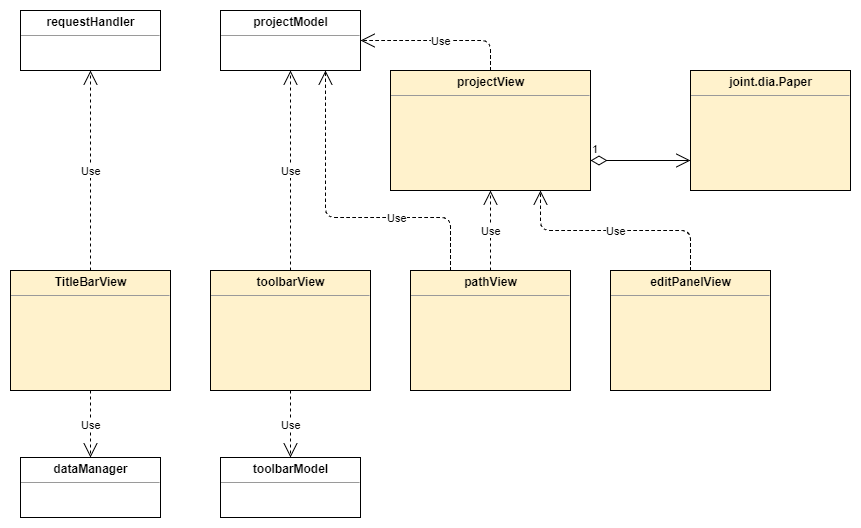
\includegraphics[scale=0.44]{Immagini/DiagrammaArchitettura/View.png}
						\caption{Architettura di View}
					\end{figure}
				Questo package non contiene dei sottopackage.
				Le classi contenute al suo interno verranno elencate qui di seguito.

				\subsubsection{SWEDesigner::Client::View::ProjectView}
					\hypertarget{SWEDesigner::Client::View::ProjectView}{}
					\begin{itemize}
						\item \textbf{Tipo}: \emph{Class};
						\item \textbf{Descrizione}: Questa classe gestisce il diagramma disegnato e le interazioni dell'utente con esso;
						\item \textbf{Padre}: \emph{Backbone.View};
						\item \textbf{Attributi}:
						\begin{itemize}
							\item \emph{model} \\
							Istanza di \hyperlink{SWEDesigner::Model::ProjectModel}{\emph{ProjectModel}} del programma;
							\item \emph{paper} \\
							Oggetto joint.dia.Paper della libreria esterna JointJS;
						\end{itemize}
						\item \textbf{Metodi}:
						\begin{itemize}
							\item \emph{resetSelectedCell(): void} \\
							Pone this.paper.selectedCell a null e genera l'evento "changed-selected-cell";
							\item \emph{mouseMoveFunction(event: JavaScriptEvent): void} \\
							Provoca la traslazione del paper nella direzione del trascinamento del mouse; \\
							Parametri:
							\begin{itemize}
								\item \emph{event: JavaScriptEvent}: Evento;
							\end{itemize}
							\item \emph{blankPointerDown(elem: CellView, event: JavaScriptEvent, x: Double, y: Double): void} \\
							Salva le correnti coordinate al click del mouse nello spazio vuoto del paper; \\
							Parametri:
							\begin{itemize}
								\item \emph{elem: CellView}: Elemento cellView;
								\item \emph{event: JavaScriptEvent}: Evento;
								\item \emph{x: Double}: Coordinata dell'asse delle ascisse;
								\item \emph{y: Double}: Coordinata dell'asse delle ordinate;
							\end{itemize}
							\item \emph{blankPointerUp(elem: CellView, event: JavaScriptEvent, x: Double, y: Double): void} \\
							Elimina le coordinate iniziali al click del mouse nello spazio vuoto del paper; \\
							Parametri:
							\begin{itemize}
								\item \emph{elem: CellView}: Elemento cellView;
								\item \emph{event: JavaScriptEvent}: Evento;
								\item \emph{x: Double}: Coordinata dell'asse delle ascisse;
								\item \emph{y: Double}: Coordinata dell'asse delle ordinate;
							\end{itemize}
							\item \emph{onMouseWheel(elem: CellView, event: JavaScriptEvent): void} \\
							Trasla verticalmente il paper effettuando uno zoom in avanti o indietro a seconda della rotazione della ruota del mouse; \\
							Parametri:
							\begin{itemize}
								\item \emph{elem: CellView}: Elemento cellView;
								\item \emph{event: JavaScriptEvent}: Evento;
							\end{itemize}
							\item \emph{render(): void} \\
							Provoca il render della projectVIew;
							\item \emph{addCell(elem: CellView, event: JavaScriptEvent, x: Double, y: Double): void} \\
							Aggiunge un nuovo elemento al graph chiamando il relativo metodo di \hyperlink{SWEDesigner::Model::ProjectModel}{\emph{ProjectModel}}; \\
							Parametri:
							\begin{itemize}
								\item \emph{elem: cellView}: Elemento CellView;
								\item \emph{event: JavaScriptEvent}: Evento;
								\item \emph{x: Double}: Coordinata dell'asse delle ascisse;
								\item \emph{y: Double}: Coordinata dell'asse delle ordinate;
							\end{itemize}
							\item \emph{deleteCell(event: JavaScriptEvent): void} \\
							Elimina un elemento dal graph chiamando il relativo metodo di ProjectModel;\\
							Parametri:
							\begin{itemize}
								\item \emph{event: JavaScriptEvent}: Evento;
							\end{itemize}
							\item \emph{unembedCell(event: JavaScriptEvent): void} \\
							Rimuove l'innestamento della cella selezionata;\\
							Parametri:
							\begin{itemize}
								\item \emph{event: JavaScriptEvent}: Evento;
							\end{itemize}
							\item \emph{pointerDownFunction(prView: \hyperlink{SWEDesigner::Client::View::projectView}{\emph{projectView}}, elem: cellView, event: JavaScriptEvent, x: double, y: double): void} \\
							Gestice l'evento generato dal click (non rilasciato) del mouse nel paper. Se viene cliccato un elemento, genera a sua volta l'evento "changed-selected-cell" gestito da \hyperlink{SWEDesigner::Client::View::EditPanelView}{\emph{EditPanelView}};\\
							Parametri:
							\begin{itemize}
								\item \emph{prView: \hyperlink{SWEDesigner::Client::View::ProjectView}{\emph{ProjectView}}}: Istanza di ProjectView;
								\item \emph{elem: cellView}: Elemento CellView;
								\item \emph{event: JavaScriptEvent}: Evento;
								\item \emph{x: Double}: Coordinata dell'asse delle ascisse;
								\item \emph{y: Double}: Coordinata dell'asse delle ordinate;
							\end{itemize}
							\item \emph{pointerUpFunction(prView: \hyperlink{SWEDesigner::Client::View::ProjectView}{\emph{ProjectView}}, elem: CellView, event: JavaScriptEvent, x: Double, y: Double): void} \\
							Gestice l'evento generato dal click (al rilascio) del mouse nel paper (rimozione di un elemento, nesting di un elemento in un'altro, collegamento di una relazione tra elementi);\\
							Parametri:
							\begin{itemize}
								\item \emph{prView: \hyperlink{SWEDesigner::Client::View::projectView}{\emph{projectView}}}: Istanza di projectView;
								\item \emph{elem: CellView}: Elemento cellView;
								\item \emph{event: JavaScriptEvent}: Evento;
								\item \emph{x: Double}: Coordinata dell'asse delle ascisse;
								\item \emph{y: Double}: Coordinata dell'asse delle ordinate;
							\end{itemize}
							\item \emph{switchIn(id: String): void} \\
							Gestisce lo switch in profondità (dall'elemento selezionato il cui id è parametro in input) invocando il relativo metodo di \hyperlink{SWEDesigner::Model::ProjectModel}{\emph{ProjectModel}};\\
							Parametri:
							\begin{itemize}
								\item \emph{id: String}: Identificativo dell'elemento;
							\end{itemize}
							\item \emph{switchOut(diagramType: String): void} \\
							Gestisce lo switch verso un diagramma (il cui tipo è parametro in input) antistante da quello corrente invocando il relativo metodo di \hyperlink{SWEDesigner::Model::ProjectModel}{\emph{ProjectModel}}.\\
							Parametri:
							\begin{itemize}
								\item \emph{diagramType: String}: Tipo di diagramma di destinazione;
							\end{itemize}
							\item \emph{deleteOperationAt(ind: Int): void} \\
							Gestisce l'eliminazione di un diagramma delle bubble invocando il relativo metodo di \hyperlink{SWEDesigner::Model::projectModel}{\emph{projectModel}}.\\
							Parametri:
							\begin{itemize}
								\item \emph{ind: Int}: Indice dell'array di operazioni del diagramma delle bubble da eliminare;
							\end{itemize}
						\end{itemize}
						\item \textbf{Relazioni con le altre classi}:
						\begin{itemize}
							\item IN \hyperlink{SWEDesigner::View::PathView}{\emph{PathView}}: gestisce l'interfaccia grafica della barra di indirizzo;
							\item IN \hyperlink{SWEDesigner::View::EditPanelView}{\emph{EditPanelView}}: gestisce l'interfaccia grafica del pannello di editing.
							\item OUT \hyperlink{SWEDesigner::Model::ProjectModel}{\emph{ProjectModel}}: si occupa di gestire la parte logica dell'editor;
							\item OUT joint.dia.Paper: gestisce l'interfaccia grafica dell'area dei diagrammi.
						\end{itemize}
					\end{itemize}
					
				\subsubsection{SWEDesigner::Client::View::TitlebarView}
					\hypertarget{SWEDesigner::Client::View::TitlebarView}{}
					\begin{itemize}
						\item \textbf{Tipo}: \emph{Class};
						\item \textbf{Descrizione}: È il componente del programma che fa la funzione di view per la barra del titolo, dove saranno collocati il menu dell’applicazione e gli shortcut;
						\item \textbf{Padre}: \emph{Backbone.View};
						\item \textbf{Attributi}:
						\begin{itemize}
							\item \emph{el: String} \\
							Il tag HTML popolato dalla Titlebar;
							\item \emph{events: Object} \\
							Gli eventi verificabili nella titlebar;
						\end{itemize}
						\item \textbf{Metodi}:
						\begin{itemize}
							\item \emph{generateJava(event: JavaScriptEvent): void} \\
							Richiede al server di generare il codice in linguaggio Java del progetto correntemente aperto invocando il rispettivo metodo di \hyperlink{SWEDesigner::Model::RequestHandler}{\emph{RequestHandler}}; \\
							Parametri:
							\begin{itemize}
								\item \emph{event: JavaScriptEvent}: Evento;
							\end{itemize}
							\item \emph{generateJavascript(event: JavaScriptEvent): void} \\
							Richiede al server di generare il codice in linguaggio JavaScript del progetto correntemente aperto invocando il rispettivo metodo di \hyperlink{SWEDesigner::Model::RequestHandler}{\emph{RequestHandler}}; \\
							Parametri:
							\begin{itemize}
								\item \emph{event: JavaScriptEvent}: Evento;
							\end{itemize}
							\item \emph{newProject(event: JavaScriptEvent): void} \\
							Crea un nuovo progetto invocando il rispettivo metodo di \hyperlink{SWEDesigner::Model::DataManager}{\emph{DataManager}} \\
							Parametri:
							\begin{itemize}
								\item \emph{event: JavaScriptEvent}: Evento;
							\end{itemize}
							\item \emph{openProject(event: JavaScriptEvent): void} \\
							Apre un progetto invocando il rispettivo metodo di \hyperlink{SWEDesigner::Model::DataManager}{\emph{DataManager}} \\
							Parametri:
							\begin{itemize}
								\item \emph{event: JavaScriptEvent}: Evento;
							\end{itemize}
							\item \emph{saveProject(event: JavaScriptEvent): void} \\
							Salva il progetto correntemente aperto invocando il rispettivo metodo di \hyperlink{SWEDesigner::Model::DataManager}{\emph{DataManager}} \\
							Parametri:
							\begin{itemize}
								\item \emph{event: JavaScriptEvent}: Evento;
							\end{itemize}
							\item \emph{saveProjectAs(event: JavaScriptEvent): void} \\
							Salva il progetto correntemente aperto con nome specificato dall'utente invocando il rispettivo metodo di \hyperlink{SWEDesigner::Model::DataManager}{\emph{DataManager}} \\
							Parametri:
							\begin{itemize}
								\item \emph{event: JavaScriptEvent}: Evento;
							\end{itemize}
						\end{itemize}
						\item \textbf{Relazioni con le altre classi}:
						\begin{itemize}
							\item OUT \hyperlink{SWEDesigner::Model::RequestHandler}{\emph{RequestHandler}}: gestisce la comunicazione con il server;
							\item OUT \hyperlink{SWEDesigner::Model::DataManager}{\emph{DataManager}}: gestisce la persistenza dei dati su file system.
						\end{itemize}
					\end{itemize}

				\subsubsection{SWEDesigner::Client::View::ToolbarView}
					\hypertarget{SWEDesigner::Client::View::ToolbarView}{}
					\begin{itemize}
						\item \textbf{Tipo}: \emph{Class};
						\item \textbf{Descrizione}: È il componente del programma che fa la funzione di view per la toolbar dove saranno collocati gli strumenti per editare i diagrammi;
						\item \textbf{Padre}: \emph{Backbone.View};
						\item \textbf{Attributi}:
						\begin{itemize}
							\item \emph{el: String} \\
							Il tag HTML popolato dalla Toolbar;
							\item \emph{events: Object} \\
							Gli eventi verificabili nella Toolbar;
						\end{itemize}
						\item \textbf{Metodi}:
						\begin{itemize}
							\item \emph{addElement(event: JavaScriptEvent): void} \\
							Aggiunge un elemento al diagramma alla selezione di uno strumento invocando il rispettivo metodo di \hyperlink{SWEDesigner::Model::ToolbarModel}{\emph{ToolbarModel}}; \\
							Parametri:
							\begin{itemize}
								\item \emph{event: JavaScriptEvent}: Evento;
							\end{itemize}
							\item \emph{initialize(): void} \\
							Inizializza ToolbarView; 
							\item \emph{render(): void} \\
							Provoca il render della toolbar in base al diagramma correntemente visualizzato; 
						\end{itemize}
						\item \textbf{Relazioni con le altre classi}:
						\begin{itemize}
							\item OUT \hyperlink{SWEDesigner::Model::ProjectModel}{\emph{ProjectModel}}: si occupa di gestire la parte logica dell'editor;
							\item OUT \hyperlink{SWEDesigner::Model::ToolbarModel}{\emph{ToolbarModel}}: si occupa di gestire la parte logica della toolbar.
						\end{itemize}
					\end{itemize}

				\subsubsection{SWEDesigner::Client::View::PathView}
					\hypertarget{SWEDesigner::Client::View::PathView}{}
					\begin{itemize}
						\item \textbf{Tipo}: \emph{Class};
						\item \textbf{Descrizione}: È il componente del programma che fa la funzione di view per il cosiddetto breadcrumb dove viene inserita la posizione corrente;
						\item \textbf{Padre}: \emph{Backbone.View};
						\item \textbf{Attributi}:
						\begin{itemize}
							\item \emph{el: String} \\
							Il tag HTML popolato dalla path;
							\item \emph{events: Object} \\
							Gli eventi verificabili nella path;
						\end{itemize}
						\item \textbf{Metodi}:
						\begin{itemize}
							\item \emph{initialize(): void} \\
							Inizializza PathView; 
							\item \emph{render(): void} \\
							Provoca il render del path in base al diagramma correntemente visualizzato; 
							\item \emph{switchDiagram(event: JavaScriptEvent): void} \\
							Metodo chiamato da evento generato. Switch verso un tipo antistante di diagramma.; \\
							Parametri:
							\begin{itemize}
								\item \emph{event: JavaScriptEvent}: Evento;
							\end{itemize}
						\end{itemize}
						\item \textbf{Relazioni con le altre classi}:
						\begin{itemize}
							\item OUT \hyperlink{SWEDesigner::Model::ProjectModel}{\emph{ProjectModel}}: si occupa di gestire la parte logica dell'editor;
							\item OUT \hyperlink{SWEDesigner::View::ProjectView}{\emph{ProjectView}}: si occupa di gestire la parte grafica del model.
						\end{itemize}
					\end{itemize}

				\subsubsection{SWEDesigner::Client::View::EditPanelView}
					\hypertarget{SWEDesigner::Client::View::EditPanelView}{}
					\begin{itemize}
						\item \textbf{Tipo}: \emph{Class};
						\item \textbf{Descrizione}: ;
						\item \textbf{Padre}: \emph{Backbone.View};
						\item \textbf{Attributi}:
						\begin{itemize}
							\item \emph{currentTemplate: Object}\\
							Il template correntemente caricato e renderizzato;
							\item \emph{el: String} \\
							Il tag HTML popolato dalla path;
							\item \emph{events: Object} \\
							Gli eventi verificabili nella path;
							\item \emph{tagname: String} \\
							Il tag HTML popolato dal pannello;
						\end{itemize}
						\item \textbf{Metodi}:
						\begin{itemize}
							\item \emph{confirmEdit(event: JavaScriptEvent): void} \\
							Metodo chiamato da evento generato, salva le modifiche apportate ad una proprietà del contenuto selezionato nel pannello; \\
							Parametri:
							\begin{itemize}
								\item \emph{event: JavaScriptEvent}: Evento;
							\end{itemize}
							\item \emph{execCommand(event: JavaScriptEvent): void} \\
							Metodo chiamato da evento generato, esegue il metodo definito dal nome dell'elemento generante l'evento sul contenuto selezionato nel pannello; \\
							Parametri:
							\begin{itemize}
								\item \emph{event: JavaScriptEvent}: Evento;
							\end{itemize}
							\item \emph{initialize(): void} \\
							Inizializza la EditPanelView; 
							\item \emph{render(): void} \\
							Provoca il render del pannello in base all'elemento del paper cliccato; 
							\item \emph{reset(): void} \\
							Provoca il reset del pannello; 
							\item \emph{saveCode(event: JavaScriptEvent): void} \\
							Metodo chiamato da evento generato, salva il codice interno ad una customBubble; \\
							Parametri:
							\begin{itemize}
								\item \emph{event: JavaScriptEvent}: Evento;
							\end{itemize}
							\item \emph{switch(event: JavaScriptEvent): void} \\
							Metodo chiamato da evento generato, esegue lo switch in profondità del tipo di diagramma; \\
							Parametri:
							\begin{itemize}
								\item \emph{event: JavaScriptEvent}: Evento;
							\end{itemize}
							\item \emph{switchDiagram(event: JavaScriptEvent): void} \\
							Metodo chiamato da evento generato, esegue lo switch verso un tipo antistante di diagramma; \\
							Parametri:
							\begin{itemize}
								\item \emph{event: JavaScriptEvent}: Evento;
							\end{itemize}
							\item \emph{unembedCell(event: JavaScriptEvent): void} \\
							Metodo chiamato da evento generato, rimuove la bubble selezionata nel pannello dall'innesto; \\
							Parametri:
							\begin{itemize}
								\item \emph{event: JavaScriptEvent}: Evento;
							\end{itemize}
						\end{itemize}
						\item \textbf{Relazioni con le altre classi}:
						\begin{itemize}
							\item OUT \hyperlink{SWEDesigner::View::ProjectView}{\emph{ProjectView}}: si occupa di gestire la parte grafica del model.
						\end{itemize}
					\end{itemize}

			\subsection{SWEDesigner::Server}
			% IMMAGINE ARCHITETTURA SERVER GENERALE
			\begin{figure}[H]\label{fig:ServerSubsystem}
				\centering
				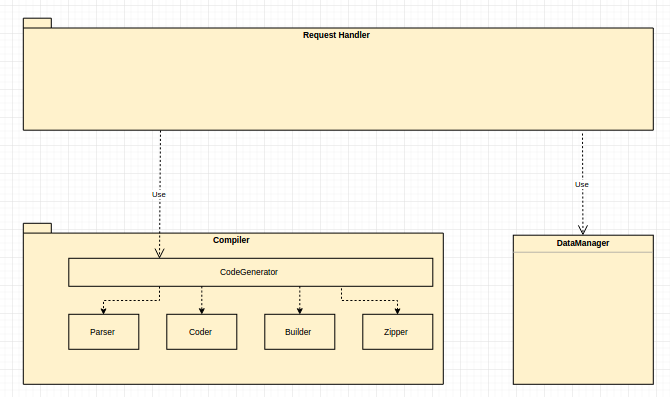
\includegraphics[scale=0.4]{Immagini/DiagrammaArchitettura/ServerSubsystem.png}
				\caption{Architettura del server}
			\end{figure}
			I package contenuti al suo interno sono:
			\begin{itemize}
				\item SWEDesigner::Server::CodeGenerator;
				\item SWEDesigner::Server::DataManager;
				\item SWEDesigner::Server::RequestHandler.
			\end{itemize}
			Questo package non contiene delle classi.
			
			\subsection{SWEDesigner::Server::CodeGenerator}
			I package contenuti al suo interno sono:
			\begin{itemize}
				\item SWEDesigner::Server::CodeGenerator::Builder;
				\item SWEDesigner::Server::CodeGenerator::Coder;
				\item SWEDesigner::Server::CodeGenerator::Parser;
				\item SWEDesigner::Server::CodeGenerator::Zipper.
			\end{itemize}
			Le classi contenute al suo interno verranno elencate qui di seguito.
			
			\subsubsection{SWEDesigner::Server::CodeGenerator::CodeGenerator}
			\hypertarget{SWEDesigner::Server::CodeGenerator::CodeGenerator}{}
			\begin{itemize}
				\item \textbf{Tipo}: \emph{Class};\\
				\item \textbf{Descrizione}: Rende disponibile la funzionalità per cui, dato un file in formato JSON che contiene le informazioni necessarie a codificare un programma, restituisce un pacchetto in formato .zip contenente i file del codice sorgente che costituiscono il programma rappresentato dal file in input. I file prodotti sono organizzati in packages, come indicato nel file JSON in input;\\
				\item \textbf{Metodi}:
				\begin{itemize}
					\item \emph{generateJsProgram(jsonProgram:JSON, nomeZip:string):void} \\ 
					Funzione statica che codifica, in Javascript, il programma corrispondente al contenuto del JSON in input e costruisce un pacchetto compresso in formato .zip contenente
					il programma codificato e strutturato in file e directory come specificato nel file JSON di input; \\
					Parametri:
					\begin{itemize}
						\item \emph{jsonProgram:JSON}: Contiene le informazioni, in formato JSON, necessarie a codificare un programma.\\
						\item \emph{nomeZip:string}: Specifica il nome con cui verrà nominato il pacchetto zip prodotto.\\
					\end{itemize}					
					\item \emph{generateJavaProgram(jsonProgram:JSON, nomeZip:string):void} \\ 
					Funzione statica che codifica, in Java, il programma corrispondente al contenuto del JSON in input e costruisce un pacchetto compresso in formato .zip contenente il programma codificato e strutturato in file e directory come specificato nel file JSON di input; \\							
					Parametri:
					\begin{itemize}
						\item \emph{jsonProgram:JSON}: Contiene le informazioni, in formato JSON, necessarie a codificare un programma.\\
						\item \emph{nomeZip:string}:ì Specifica il nome con cui verrà nominato il pacchetto zip prodotto.\\
					\end{itemize}
				\end{itemize}				
				\item \textbf{Relazioni con le altre classi:}
				\begin{itemize}
					\item OUT \hyperlink{SWEDesigner::Server::CodeGenerator::Parser::Parser}{\emph{SWEDesigner::Server::CodeGenerator::Parser::Parser}}\\
					\item OUT \hyperlink{SWEDesigner::Server::CodeGenerator::Coder::JavaCoder}{\emph{SWEDesigner::Server::CodeGenerator::Coder::JavaCoder}}\\
					\item OUT \hyperlink{SWEDesigner::Server::CodeGenerator::Coder::JavascriptCoder}{\emph{SWEDesigner::Server::CodeGenerator::Coder::JavascriptCoder}}\\
					\item OUT \hyperlink{SWEDesigner::Server::CodeGenerator::Builder::Builder}{\emph{SWEDesigner::Server::CodeGenerator::Builder::Builder}}\\
					\item OUT \hyperlink{SWEDesigner::Server::CodeGenerator::Zipper::Zipper}{\emph{SWEDesigner::Server::CodeGenerator::Zipper::Zipper}}\\
					\item IN \hyperlink{SWEDesigner::Server::RequestHandler::RequestHandler}{\emph{SWEDesigner::Server::RequestHandler::RequestHandler}}\\
				\end{itemize}	
			\end{itemize}
			
				
			
			
			%%%%%%%%%%%%%%%%%%%%%%%%%%%%%%%%%%%%%%%%%%%%%%%%%%%%%%%%%%%%%%%%%%%%%%%%%%%%%%%%%%%%%%%%%%%%%%%%%%%%%%%%%%%%%%%%%%%%%%%%%%%%%%%%%%%%%%%%%%%%%%%%%%%%%%%%%%%%%%%%%%%%%%%%
			
			\subsection{SWEDesigner::Server::CodeGenerator::Parser}
			Questo package non contiene dei sottopackage.
			Le classi contenute al suo interno verranno elencate qui di seguito.
			
			\subsubsection{SWEDesigner::Server::CodeGenerator::Parser::Parser}
			\hypertarget{SWEDesigner::Server::CodeGenerator::Parser::Parser}{}
			\begin{itemize}
				\item \textbf{Tipo}: \emph{Class};
				\item \textbf{Descrizione}: Rende disponibile la funzionalità, dato un file JSON valido in input, di ottenere un oggetto contenente le informazioni che costituiscono il file JSON di input;\\
				\item \textbf{Metodi}:
				\begin{itemize}
					\item \emph{parse(jsonFile:JSON):Object} \\ 
					Trasforma il file JSON ricevuto in input in un oggetto Javascript contenente tutte le sue informazioni; \\
					Parametri:
					\begin{itemize}
						\item \emph{jsonFile:JSON} Contiene le informazioni, in formato JSON, necessarie a codificare un programma.
					\end{itemize}
				\end{itemize}
				
				\item \textbf{Relazioni con le altre classi:}
				\begin{itemize}
					\item IN \hyperlink{SWEDesigner::Server::CodeGenerator::CodeGenerator}{\emph{SWEDesigner::Server::CodeGenerator::CodeGenerator}}
				\end{itemize}	
			\end{itemize}
			
			%%%%%%%%%%%%%%%%%%%%%%%%%%%%%%%%%%%%%%%%%%%%%%%%%%%%%%%%%%%%%%%%%%%%%%%%%%%%%%%%%%%%%%%%%%%%%%%%%%%%%%%%%%%%%%%%%%%%%%%%%%%%%%%%%%%%%%%%%%%%%%%%%%%%%%%%%%%%%%%%%%%%%%%%
			
			
			\subsection{SWEDesigner::Server::CodeGenerator::Coder}
			% IMMAGINE ARCHITETTURA CODER
			\begin{figure}[H]\label{fig:Coder}
				\centering
				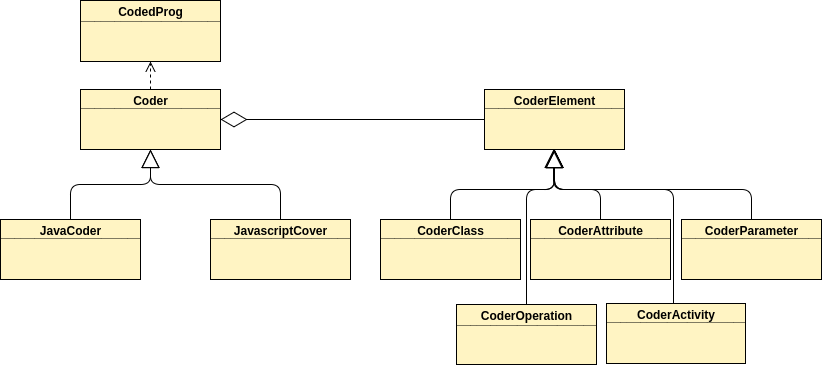
\includegraphics[scale=0.46]{Immagini/DiagrammaArchitettura/Coder.png}
				\caption{Architettura di Coder}
			\end{figure}
			
			Questo package non contiene dei sottopackage.\\
			Le classi contenute al suo interno verranno elencate qui di seguito.
			
			%		\subsubsection{SWEDesigner::Server::CodeGenerator::Coder::Coder}
			%		Componente che funge da interfaccia alle operazioni di codifica di una stringa, in formato JSON che rappresenta un programma valido; tali operazioni permettono di ottenere un %	oggetto contenente il codice sorgente, in Java o Javascript, corrispondente alla stringa in input.\\
			%		FAN-IN:
			%		\begin{itemize}
			%			\item JavaCoder: si occupa di trasformare un oggetto JSON ricevuto in input in un oggetto contenente il codice sorgente scritto in java;
			%			\item JavaScriptCoder: si occupa di trasformare un oggetto JSON ricevuto in input in un oggetto contenente il codice sorgente scritto in javascript.
			%		\end{itemize}
			%		FAN-OUT:
			%			\item CoderElement: componente astratto che offre la funzionalità che permette di associare ad ogni stringa contenuta nel file JSON il corrispondente codice sorgente.
			%		\end{itemize}
			
			\subsubsection{SWEDesigner::Server::CodeGenerator::Coder::JavaCoder}
			\hypertarget{SWEDesigner::Server::CodeGenerator::Coder::JavaCoder}{}
			\begin{itemize}
				\item \textbf{Tipo}: \emph{Class};
				\item \textbf{Descrizione}: Rende disponibile la funzionalità, dato un oggetto in input che che contiene le informazioni necessarie a codificare un programma, di ottenere un oggetto contenente il codice sorgente, in linguaggio Java, corrispondente all'oggetto in input;\\
				\item \textbf{Metodi}:
				\begin{itemize}
					\item \emph{coderParameters(operationObj:Object):string} \\ 
					Riceve in input operationObj, un oggetto che contiene le informazioni necessarie a codificare una operazione; 
					restituisce la stringa del codice sorgente, in Java, della lista dei parametri dell'operazione operationObj di input; \\
					Parametri:
					\begin{itemize}
						\item \emph{operationObj:Object} Contiene le informazioni necessarie a codificare una operazione.
					\end{itemize}
					
					\item \emph{coderAttributes(classObj:Object):string} \\ 
					Riceve in input classObj, un oggetto che contiene le informazioni necessarie a codificare una classe; 
					restituisce la stringa del codice sorgente, in Java, di tutti gli attributi della classe classObj di input; \\
					Parametri:
					\begin{itemize}
						\item \emph{classObj:Object} Contiene le informazioni necessarie a codificare una classe.
					\end{itemize}
					
					\item \emph{coderOperations(classObj,operations):string} \\ 
					Riceve in input classObj, un oggetto che le informazioni necessarie a codificare una classe; 
					restituisce la stringa del codice sorgente, in Java, relativa alla definizione e implementazione di tutte le operazioni di classObj di input; \\
					Parametri:
					\begin{itemize}
						\item \emph{classObj:Object} Contiene le informazioni necessarie a codificare una classe;
						\item \emph{operations:Object} Contiene le informazioni necessarie a codificare l'implementazione di tutte le operazioni di classObj.
					\end{itemize}
					
					\item \emph{getCodedProgram(parsedProgram:Object):CodedProgram} \\ 
					Riceve in input parsedProgram, un oggetto che contiene le informazioni necessarie a codificare un programma; 
					restituisce un oggetto istanza di CodedProgram, contente il codice sorgente in Java di tutte le classi presenti nell'oggetto 
					parsedProgram di input; \\
					Parametri:
					\begin{itemize}
						\item \emph{parsedProgram:Object} Contiene le informazioni necessarie a codificare un programma.
					\end{itemize}
				\end{itemize}
				
				\item \textbf{Relazioni con le altre classi:}
				\begin{itemize}
					\item IN \hyperlink{SWEDesigner::Server::CodeGenerator::CodeGenerator}{\emph{SWEDesigner::Server::CodeGenerator::CodeGenerator}}
				\end{itemize}	
			\end{itemize}
			
			\subsubsection{SWEDesigner::Server::CodeGenerator::Coder::JavascriptCoder}
			\hypertarget{SWEDesigner::Server::CodeGenerator::Coder::JavascriptCoder}{}
			\begin{itemize}
				\item \textbf{Tipo}: \emph{Class};
				\item \textbf{Descrizione}: Rende disponibile la funzionalità, dato un oggetto in input che contiene le informazioni necessarie a codificare un programma, di ottenere un oggetto contenente il codice sorgente, in linguaggio Javascript, corrispondente all'oggetto in input;\\
				\item \textbf{Metodi}:
				\begin{itemize}
					\item \emph{coderParameters(operationObj:Object):string} \\ 
					Riceve in input operationObj, un oggetto che contiene le informazioni necessarie a codificare una operazione; 
					restituisce la stringa del codice sorgente, in Javascript, della lista dei parametri dell'operazione operationObj di input; \\
					Parametri:
					\begin{itemize}
						\item \emph{operationObj:Object} Contiene le informazioni necessarie a codificare una operazione.
					\end{itemize}
					
					\item \emph{coderInstanceAttributes(classObj:Object):string} \\ 
					Riceve in input classObj, un oggetto che contiene le informazioni necessarie a codificare una classe; 
					restituisce la stringa del codice sorgente, in Javascript, di tutti gli attributi non statici della classe classObj di input; \\
					Parametri:
					\begin{itemize}
						\item \emph{classObj:Object} Contiene le informazioni necessarie a codificare una classe.
					\end{itemize}
					
					\item \emph{coderInstanceOperations(classObj,operations):string} \\ 
					Riceve in input classObj, un oggetto che le informazioni necessarie a codificare una classe; 
					restituisce la stringa del codice sorgente, in Javascript, relativa alla definizione e implementazione di tutte le operazioni non statiche di classObj di input; \\
					Parametri:
					\begin{itemize}
						\item \emph{classObj:Object} Contiene le informazioni necessarie a codificare una classe;
						\item \emph{operations:Object} Contiene le informazioni necessarie a codificare l'implementazione di tutte le operazioni di classObj.
					\end{itemize}
					
					\item \emph{coderStaticAttributes(classObj:Object):string} \\ 
					Riceve in input classObj, un oggetto che contiene le informazioni necessarie a codificare una classe; 
					restituisce la stringa del codice sorgente, in Javascript, di tutti gli attributi statici della classe classObj di input; \\
					Parametri:
					\begin{itemize}
						\item \emph{classObj:Object} Contiene le informazioni necessarie a codificare una classe.
					\end{itemize}
					
					\item \emph{coderStaticOperations(classObj,operations):string} \\ 
					Riceve in input classObj, un oggetto che le informazioni necessarie a codificare una classe; 
					restituisce la stringa del codice sorgente, in Javascript, relativa alla definizione e implementazione di tutte le operazioni statiche di classObj di input; \\
					Parametri:
					\begin{itemize}
						\item \emph{classObj:Object} Contiene le informazioni necessarie a codificare una classe;
						\item \emph{operations:Object} Contiene le informazioni necessarie a codificare l'implementazione di tutte le operazioni di classObj.
					\end{itemize}
					
					\item \emph{getCodedProgram(parsedProgram:Object):CodedProgram} \\ 
					Riceve in input parsedProgram, un oggetto che contiene le informazioni necessarie a codificare un programma; 
					restituisce un oggetto istanza di CodedProgram, contente il codice sorgente in Javascript di tutte le classi presenti nell'oggetto 
					parsedProgram di input; \\
					Parametri:
					\begin{itemize}
						\item \emph{parsedProgram:Object} Contiene le informazioni necessarie a codificare un programma.
					\end{itemize}
				\end{itemize}
				
				\item \textbf{Relazioni con le altre classi:}
				\begin{itemize}
					\item IN \hyperlink{SWEDesigner::Server::CodeGenerator::CodeGenerator}{\emph{SWEDesigner::Server::CodeGenerator::CodeGenerator}}
				\end{itemize}	
			\end{itemize}
			
			
			%		\subsubsection{SWEDesigner::Server::CodeGenerator::Coder::CoderClass}
			%		È il componente che mette a disposizione la funzionalità, data una stringa in input in formato JSON che rappresenta una classe valida, di ottenere il corrispondente codice %		sorgente di tale classe.\\
			%		Non ci sono dipendenze IN.\\
			%		FAN-OUT:
			%		\begin{itemize}
			%			\item CoderElement: componente astratto che offre la funzionalità che permette di associare ad ogni stringa contenuta nel file JSON il corrispondente codice sorgente.
			%		\end{itemize}
			
			\subsubsection{SWEDesigner::Server::CodeGenerator::Coder::CoderOperation}
			\hypertarget{SWEDesigner::Server::CodeGenerator::Coder::CoderOperation}{}
			\begin{itemize}
				\item \textbf{Tipo}: \emph{Class};
				\item \textbf{Descrizione}: Rende disponibile la funzionalità che permette di codificare l'intestazione dell'operazione corrispondente al contenuto dell'oggetto operationObj di input; \\
				\item \textbf{Metodi}:
				\begin{itemize}
					\item \emph{codeElementJava(operationObj:Object):string} \\ 
					Riceve in input operationObj, un oggetto che contiene le informazioni necessarie a codificare una operazione; 
					restituisce la stringa codice sorgente in Java relativa all'intestazione dell'operazione operationObj di input; \\
					Parametri:
					\begin{itemize}
						\item \emph{operationObj:Object} Contiene le informazioni necessarie a codificare una operazione.
					\end{itemize}
					
					
					
					\item \emph{codeElementJavascript(operationObj:Object, className:string):string} \\ 
					Riceve in input operationObj, un oggetto che contiene le informazioni necessarie a codificare una operazione; 
					restituisce la stringa codice sorgente in Javascript relativa all'intestazione dell'operazione operationObj di input; \\
					Parametri:
					\begin{itemize}
						\item \emph{operationObj:Object} Contiene le informazioni necessarie a codificare una operazione;
						\item \emph{className:string} Il nome della classe che possiede l'operazione operationObj. Necessaria solo sè tale operazione è statica;
					\end{itemize}
				\end{itemize}
				
				\item \textbf{Relazioni con le altre classi:}
				\begin{itemize}
					\item IN \hyperlink{SWEDesigner::Server::CodeGenerator::Coder::JavascriptCoder}{\emph{SWEDesigner::Server::CodeGenerator::Coder::JavascriptCoder}}
					\item IN \hyperlink{SWEDesigner::Server::CodeGenerator::Coder::JavaCoder}{\emph{SWEDesigner::Server::CodeGenerator::Coder::JavaCoder}}
				\end{itemize}	
			\end{itemize}
			
			
			
			\subsubsection{SWEDesigner::Server::CodeGenerator::Coder::CoderParameter}
			\hypertarget{SWEDesigner::Server::CodeGenerator::Coder::CoderParameter}{}
			\begin{itemize}
				\item \textbf{Tipo}: \emph{Class};
				\item \textbf{Descrizione}: Rende disponibile la funzionalità che permette di codificare un parametro, corrispondente al contenuto dell'oggetto parameterObj di input;\\
				\item \textbf{Metodi}:
				\begin{itemize}
					\item \emph{codeElementJava(parameterObj:Object):string} \\ 
					Riceve in input parameterObj, un oggetto che contiene le informazioni necessarie a codificare un parametro di operazione; 
					restituisce la stringa codice sorgente in Java relativa al parametro parameterObj di input; \\
					Parametri:
					\begin{itemize}
						\item \emph{parameterObj:Object} Contiene le informazioni necessarie a codificare un parametro di operazione.
					\end{itemize}
					
					
					
					\item \emph{codeElementJavascript(parameterObj:Object):string} \\ 
					Riceve in input parameterObj, un oggetto che contiene le informazioni necessarie a codificare un parametro di operazione; 
					restituisce la stringa codice sorgente in Javascript relativa al parametro parameterObj di input; \\
					Parametri:
					\begin{itemize}
						\item \emph{parameterObj:Object} Contiene le informazioni necessarie a codificare un parametro di operazione.
					\end{itemize}
				\end{itemize}
				
				\item \textbf{Relazioni con le altre classi:}
				\begin{itemize}
					\item IN \hyperlink{SWEDesigner::Server::CodeGenerator::Coder::JavascriptCoder}{\emph{SWEDesigner::Server::CodeGenerator::Coder::JavascriptCoder}}
					\item IN \hyperlink{SWEDesigner::Server::CodeGenerator::Coder::JavaCoder}{\emph{SWEDesigner::Server::CodeGenerator::Coder::JavaCoder}}
				\end{itemize}	
			\end{itemize}
			
			
			\subsubsection{SWEDesigner::Server::CodeGenerator::Coder::CoderAttribute}
			\hypertarget{SWEDesigner::Server::CodeGenerator::Coder::CoderAttribute}{}
			\begin{itemize}
				\item \textbf{Tipo}: \emph{Class};
				\item \textbf{Descrizione}: Rende disponibile la funzionalità che permette di codificare un attributo corrispondente al contenuto dell'oggetto attributeObj di input;\\
				\item \textbf{Metodi}:
				\begin{itemize}
					\item \emph{codeElementJava(attributeObj:Object):string} \\ 
					Riceve in input attributeObj, un oggetto che contiene le informazioni necessarie a codificare un attributo di classe; 
					restituisce la stringa codice sorgente in Java relativa all'attributo attributeObj di input; \\
					Parametri:
					\begin{itemize}
						\item \emph{attributeObj:Object} Contiene le informazioni necessarie a codificare un attributo di classe.
					\end{itemize}
					
					
					
					\item \emph{codeElementJavascript(attributeObj:Object, className:string):string} \\ 
					Riceve in input attributeObj, un oggetto che contiene le informazioni necessarie a codificare un attributo; 
					restituisce la stringa codice sorgente in Javascript relativa all'attributo attributeObj di input; \\
					Parametri:
					\begin{itemize}
						\item \emph{attributeObj:Object} Contiene le informazioni necessarie a codificare un attributo di classe;
						\item \emph{className:string} Il nome della classe che possiede l'attributo attributeObj. Necessaria solo sè tale attributo è statico;
					\end{itemize}
				\end{itemize}
				
				\item \textbf{Relazioni con le altre classi:}
				\begin{itemize}
					\item IN \hyperlink{SWEDesigner::Server::CodeGenerator::Coder::JavascriptCoder}{\emph{SWEDesigner::Server::CodeGenerator::Coder::JavascriptCoder}}
					\item IN \hyperlink{SWEDesigner::Server::CodeGenerator::Coder::JavaCoder}{\emph{SWEDesigner::Server::CodeGenerator::Coder::JavaCoder}}
				\end{itemize}	
			\end{itemize}
			
			
			
			\subsubsection{SWEDesigner::Server::CodeGenerator::Coder::CoderActivity}
			\hypertarget{SWEDesigner::Server::CodeGenerator::Coder::CoderActivity}{}
			\begin{itemize}
				\item \textbf{Tipo}: \emph{Class};
				\item \textbf{Descrizione}: Rende disponibile la funzionalità che permette di codificare l'implementazione di un'operazione, corrispondente al contenuto dell'oggetto activityObj di input; \\
				\item \textbf{Metodi}:
				\begin{itemize}
					\item \emph{getBubbleLinks(activityObj:Object):Array} \\ 
					Estrae, per ogni elemento in activityObj, le informazioni relative al collegamento con un'altro elemento (se esiste) contenuto in ActivityObj e
					le inserisce in un array che viene restituito; \\
					Parametri:
					\begin{itemize}
						\item \emph{activityObj:Object} Contiene le informazioni necessarie a codificare l'implementazione di un operazione. E costituito da elementi ognuno contenente le informazioni necessarie a codificare una porzione dell'implementazione dell'operazione.
					\end{itemize}
					
					\item \emph{getBubbleId(bubbleId:string, activityObj:Object):Object} \\ 
					Ritorna la bubble (oggetto contenente le informazioni necessarie a codificare una porzione dell'implementazione di activityObj) contenuta in activityObj e il cui identificativo corrisponde al bubbleId di input; \\
					Parametri:
					\begin{itemize}
						\item \emph{bubbleId:string} Stringa identificativa della bubble che si vuole ottenere;
						\item \emph{activityObj:Object} Contiene le informazioni necessarie a codificare l'implementazione di un operazione. E costituito da elementi (bubble) ognuno contenente le informazioni necessarie a codificare una porzione dell'implementazione dell'operazione.
					\end{itemize}
					
					\item \emph{getNextBubble(bubbleObj:Object, activityObj:Object):Object} \\ 
					Ritorna la bubble (oggetto contenente le informazioni necessarie a codificare una porzione dell'implementazione di activityObj) contenuta in activityObj, successiva alla bubble di input anch'essa contenuta in activityObj; \\
					Parametri:
					\begin{itemize}
						\item \emph{bubbleObj:Object} Contiene le informazioni necessarie a codificare una porzione dell'implementazione di un'operazione;
						\item \emph{activityObj:Object} Contiene le informazioni necessarie a codificare l'implementazione di un operazione. E costituito da elementi (bubble) ognuno contenente le informazioni necessarie a codificare una porzione dell'implementazione dell'operazione.
					\end{itemize}	
					
					\item \emph{getStartBubble(bubbleArray:Array, parent:string):Object} \\ 
					Ritorna la bubble (oggetto contenente le informazioni necessarie a codificare una porzione dell'implementazione di una operazione) contenuta in bubbleArray, corrispondente alla bubble iniziale, ovvero la bubble da cui comincia la sotto attività rappresentata da bubbleArray; \\
					Parametri:
					\begin{itemize}
						\item \emph{bubbleArray:Array} Contiene le informazioni necessarie a codificare una sotto attività di un'operazione;
						\item \emph{parent:string} Contiene l'identificativo della bubble in cui sono innestate le bubble presenti in bubbleArray.	
					\end{itemize}		
					
					\item \emph{codeEmbeddedBubbles(bubbleObj:Object, activityObj:Object):Object} \\ 
					Codifica la bubbleObj (oggetto contenente le informazioni necessarie a codificare una porzione dell'implementazione di una operazione) di input e tutte le bubble innestate in essa; tale bubbleObj dev'essere contenuta in activityObj \\
					Parametri:
					\begin{itemize}
						\item \emph{bubbleObj:Object} Contiene le informazioni necessarie a codificare una porzione dell'implementazione di un'operazione;
						\item \emph{activityObj:Object} Contiene le informazioni necessarie a codificare l'implementazione di un operazione. E costituito da elementi (bubble) ognuno contenente le informazioni necessarie a codificare una porzione dell'implementazione dell'operazione.
					\end{itemize}
					
					\item \emph{codeBubble(bubbleObj:Object, activityObj:Object, parent:string):Object} \\ 
					Codifica la bubbleObj (oggetto contenente le informazioni necessarie a codificare una porzione dell'implementazione di una operazione) di input; tale bubbleObj dev'essere contenuta in activityObj \\
					Parametri:
					\begin{itemize}
						\item \emph{bubbleObj:Object} Contiene le informazioni necessarie a codificare una porzione dell'implementazione di un'operazione;
						\item \emph{activityObj:Object} Contiene le informazioni necessarie a codificare l'implementazione di un operazione. E costituito da elementi (bubble) ognuno contenente le informazioni necessarie a codificare una porzione dell'implementazione dell'operazione.
						\item \emph{parent:string} Contiene l'identificativo della bubble in cui è innestata la bubbleObj di input.
					\end{itemize}
					
					\item \emph{codeElementJava(activityObj:Object):string} \\ 
					Riceve in input activityObj, un oggetto che contiene le informazioni necessarie a codificare l'implementazione di un operazione; 
					restituisce la stringa codice sorgente in Java corrispondente all'implementazione della activityObj di input; \\
					Parametri:
					\begin{itemize}
						\item \emph{activityObj:Object} Contiene le informazioni necessarie a codificare l'implementazione di un operazione. E costituito da elementi (bubble) ognuno contenente le informazioni necessarie a codificare una porzione dell'implementazione dell'operazione.
					\end{itemize}
					
					
					\item \emph{codeElementJavascript(activityObj:Object):string} \\ 
					Riceve in input activityObj, un oggetto che contiene le informazioni necessarie a codificare l'implementazione di un operazione; 
					restituisce la stringa codice sorgente in Javascript corrispondente all'implementazione della activityObj di input; \\
					Parametri:
					\begin{itemize}
						\item \emph{activityObj:Object} Contiene le informazioni necessarie a codificare l'implementazione di un operazione. E costituito da elementi (bubble) ognuno contenente le informazioni necessarie a codificare una porzione dell'implementazione dell'operazione.
					\end{itemize}
				\end{itemize}
				
				\item \textbf{Relazioni con le altre classi:}
				\begin{itemize}
					\item IN \hyperlink{SWEDesigner::Server::CodeGenerator::Coder::JavascriptCoder}{\emph{SWEDesigner::Server::CodeGenerator::Coder::JavascriptCoder}}
					\item IN \hyperlink{SWEDesigner::Server::CodeGenerator::Coder::JavaCoder}{\emph{SWEDesigner::Server::CodeGenerator::Coder::JavaCoder}}
				\end{itemize}	
			\end{itemize}
			
			
			\subsubsection{SWEDesigner::Server::CodeGenerator::Coder::CodedProg}
			\hypertarget{SWEDesigner::Server::CodeGenerator::Coder::CodedProg}{}
			\begin{itemize}
				\item \textbf{Tipo}: \emph{Class};
				\item \textbf{Descrizione}: È il componente che contiene il codice sorgente prodotto dal Coder; \\
				\item \textbf{Attributi}:
				\begin{itemize}
					\item \emph{\_classes: Array}: Array contenente le informazioni di ogni classe codificata dal Coder. Tali informazioni comprendono il nome della classe, il suo codice sorgente, il nome del package in cui è contenuta e l'array delle dipendenze OUT;
				\end{itemize}
				\item \textbf{Metodi}:
				\begin{itemize}
					\item \emph{add(\_class:Object):void} \\ 
					Inserisce nell'array \_classes le informazioni della classe \_class codificata dal Coder; \\
					Parametri:
					\begin{itemize}
						\item \emph{\_class:Object} Contiene il nome della classe, il suo codice sorgente, il nome del package in cui è contenuta e l'array delle dipendenze OUT.
					\end{itemize}
					
					\item \emph{getSource(i:int):string} \\ 
					Restituisce il codice sorgente della classe contenuta nell'attributo \_classes all'indice i; \\
					Parametri:
					\begin{itemize}
						\item \emph{i:int} Indice della classe, contenuta nell'attributo \_classes, di cui si vuole il codice sorgente;
					\end{itemize}
				\end{itemize}
				
				\item \textbf{Relazioni con le altre classi:}
				\begin{itemize}
					\item IN \hyperlink{SWEDesigner::Server::CodeGenerator::Coder::JavascriptCoder}{\emph{SWEDesigner::Server::CodeGenerator::Coder::JavascriptCoder}}
					\item IN \hyperlink{SWEDesigner::Server::CodeGenerator::Coder::JavaCoder}{\emph{SWEDesigner::Server::CodeGenerator::Coder::JavaCoder}}
				\end{itemize}	
			\end{itemize}
			
			
			%		\subsubsection{SWEDesigner::Server::CodeGenerator::Coder::CoderElement}
			%		Componente astratta che offre la funzionalità di ottenere, data una stringa in input in formato JSON che rappresenta un elemento di classe valido, il corrispondente codice 	sorgente, in Java o Javascript.\\
			%		FAN-IN:
			%		\begin{itemize}
			%			\item Coder: componente che funge da interfaccia alle operazioni di codifica di una stringa permettendo quindi di trasformare le informazioni del file in formato JSON in codice sorgente;
			%			\item CoderClass: componente che permette data una stringa in input in formato JSON che rappresenta un diagramma delle classi valido, di ottenere il corrispondente codice sorgente di tale classe;
			%			\item CoderOperations: componente che permette data una stringa in input in formato JSON che rappresenta un'operazione valida, di ottenere il corrispondente codice sorgente di tale operazione;
			%			\item CoderAttributes: componente che permette data una stringa in input in formato JSON che rappresenta un attributo valido, di ottenere il corrispondente codice sorgente di tale attributo;
			%			\item CoderActivity: componente che permette data una stringa in input in formato JSON che rappresenta un diagramma delle attività valido, di ottenere il corrispondente codice sorgente di tale attività;
			%			\item CoderParameter: componente che permette data una stringa in input in formato JSON che rappresenta un parametro valido, di ottenere il corrispondente codice sorgente di tale parametro.
			%		\end{itemize}
			%		Non ci sono dipendenze OUT.
			
			%%%%%%%%%%%%%%%%%%%%%%%%%%%%%%%%%%%%%%%%%%%%%%%%%%%%%%%%%%%%%%%%%%%%%%%%%%%%%%%%%%%%%%%%%%%%%%%%%%%%%%%%%%%%%%%%%%%%%%%%%%%%%%%%%%%%%%%%%%%%%%%%%%%%%%%%%%%%%%%%%%%%%%%%
			
			\subsection{SWEDesigner::Server::CodeGenerator::Builder}
			Questo package non contiene dei sottopackage.\\
			Le classi contenute al suo interno verranno elencate qui di seguito.
			
			
			\subsubsection{SWEDesigner::Server::CodeGenerator::Builder::Builder}
			\hypertarget{SWEDesigner::Server::CodeGenerator::Builder::Builder}{}
			\begin{itemize}
				\item \textbf{Tipo}: \emph{Class};
				\item \textbf{Descrizione}: Rende disponibile la funzionalità che permette di creare su disco la directory contenente il programma corrispondente all'oggetto program di tipo CodedProgram; \\
				\item \textbf{Attributi}:
				\begin{itemize}
					\item \emph{generalPath: string}: Contiene il path alla directory dove vengono creati tutti i programmi (directories, file sorgenti, ...);
				\end{itemize}
				\item \textbf{Metodi}:
				\begin{itemize}
					\item \emph{deleteFolderRecursive(path:string):void} \\ 
					Rimuove la directory passata in input se esistente e tutto il suo contenuto ricorsivamente; \\
					Parametri:
					\begin{itemize}
						\item \emph{path:string} Il percorso alla directory da rimuovere.
					\end{itemize}
					
					\item \emph{mkJavaFile(progDir:string, name:string, pkg:string, dependencies:Array, source:string):void} \\ 
					Crea un file sorgente in Java e/o scrive ulteriore codice in append se già esistente; \\
					Parametri:
					\begin{itemize}
						\item \emph{progDir:string} La directory indicante dove creare i file sorgenti del programma;
						\item \emph{name:string} Il nome del file;
						\item \emph{pkg:string} Il package in cui è contenuto il file;
						\item \emph{dependencies:Array} L'array delle dipendenze del package;
						\item \emph{source:string} Il codice sorgente da scrivere nel file;
					\end{itemize}
					
					\item \emph{mkJavascriptFile(progDir:string, name:string, pkg:string, dependencies:Array, source:string):void} \\ 
					Crea un file sorgente in Javascript e/o scrive ulteriore codice in append se già esistente; \\
					Parametri:
					\begin{itemize}
						\item \emph{progDir:string} La directory indicante dove creare i file sorgenti del programma;
						\item \emph{name:string} Il nome del file;
						\item \emph{pkg:string} Il package in cui è contenuto il file;
						\item \emph{dependencies:Array} L'array delle dipendenze del package;
						\item \emph{source:string} Il codice sorgente da scrivere nel file;
					\end{itemize}
					
					\item \emph{javaBuild(program:CodedProgram):Object} \\ 
					Crea directory e file su disco contenente il programma in linguaggio java corrispondente all'oggetto program di input di tipo CodedProgram;; \\
					Parametri:
					\begin{itemize}
						\item \emph{program:CodedProgram} L'oggetto che contiene il codice sorgente prodotto dal Coder;.
					\end{itemize}
					
					\item \emph{javascriptBuild(program:CodedProgram):Object} \\ 
					Crea directory e file su disco contenente il programma in linguaggio javascript corrispondente all'oggetto program di input di tipo CodedProgram;; \\
					Parametri:
					\begin{itemize}
						\item \emph{program:CodedProgram} L'oggetto che contiene il codice sorgente prodotto dal Coder;.
					\end{itemize}
				\end{itemize}
				
				\item \textbf{Relazioni con le altre classi:}
				\begin{itemize}
					\item IN \hyperlink{SWEDesigner::Server::CodeGenerator::CodeGenerator}{\emph{SWEDesigner::Server::CodeGenerator::CodeGenerator}}
				\end{itemize}	
			\end{itemize}
			
			
			
			%%%%%%%%%%%%%%%%%%%%%%%%%%%%%%%%%%%%%%%%%%%%%%%%%%%%%%%%%%%%%%%%%%%%%%%%%%%%%%%%%%%%%%%%%%%%%%%%%%%%%%%%%%%%%%%%%%%%%%%%%%%%%%%%%%%%%%%%%%%%%%%%%%%%%%%%%%%%%%%%%%%%%%%%
			
			
			\subsection{SWEDesigner::Server::CodeGenerator::Zipper}
			Questo package non contiene dei sottopackage.\\
			Le classi contenute al suo interno verranno elencate qui di seguito.
			
			\subsubsection{SWEDesigner::Server::CodeGenerator::Zipper::Zipper}
			\hypertarget{SWEDesigner::Server::CodeGenerator::Builder::Builder}{}
			\begin{itemize}
				\item \textbf{Tipo}: \emph{Class};
				\item \textbf{Descrizione}: Rende disponibile la funzionalità che permette di creare un pacchetto in formato zip della directory specificata in input; \\
				\item \textbf{Metodi}:
				\begin{itemize}
					\item \emph{mkJavaFile(progDir:string, name:string, pkg:string, dependencies:Array, source:string):void} \\ 
					Crea un file sorgente in Java e/o scrive ulteriore codice in append se già esistente; \\
					Parametri:
					\begin{itemize}
						\item \emph{name:string} Il nome dell'archivio da creare;
						\item \emph{namepath:string} Il percorso alla directory del progetto da comprimere;
						\item \emph{callback:function} Callback di risposta;
					\end{itemize}
				\end{itemize}
				
				\item \textbf{Relazioni con le altre classi:}
				\begin{itemize}
					\item IN \hyperlink{SWEDesigner::Server::CodeGenerator::CodeGenerator}{\emph{SWEDesigner::Server::CodeGenerator::CodeGenerator}}
				\end{itemize}	
			\end{itemize}
			
			
			\subsection{SWEDesigner::Server::DataManager}
			Questo package non contiene dei sottopackage.\\
			Le classi contenute al suo interno verranno elencate qui di seguito.
			\subsubsection{SWEDesigner::Server::DataManager::DataManager}
			\hypertarget{SWEDesigner::Server::DataManager::DataManager}{}
			\begin{itemize}
				\item \textbf{Tipo}: \emph{Class};
				\item \textbf{Descrizione}: Espone le funzionalità che permettono di interagire con il database delle bubbles; \\
				\item \textbf{Attributi}:
				\begin{itemize}
					\item \emph{host\_:string}: L'hostname del database a cui connettersi;
					\item \emph{user:string}: L'username per il login al database;
					\item \emph{password:string}: La password per il login al database ;
					\item \emph{database:string}: Il nome del database a cui connettersi;
					\item \emph{connection:Object}: La connessione al database;
				\end{itemize}
				\item \textbf{Metodi}:
				\begin{itemize}
					\item \emph{setConnection(host:string, user:string, psw:string, db:string):void} \\ 
					Setta gli attributi necessari a creare una connessione; \\
					Parametri:
					\begin{itemize}
						\item \emph{host\_:string}: L'hostname del database a cui connettersi;
						\item \emph{user:string}: L'username per il login al database;
						\item \emph{psw:string}: La password per il login al database ;
						\item \emph{db:string}: Il nome del database a cui connettersi;
					\end{itemize}
					
					\item \emph{\_startConnection():void} \\ 
					Inizializza l'attributo connection e esegue la connessione al database; \\
					
					\item \emph{insertBubble(name:string, source:string, language:string, descr:string):void} \\ 
					Inserisce una nuova bubble nel database; \\
					Parametri:
					\begin{itemize}
						\item \emph{name:string}: Attributo 'Name' della bubble da inserire;
						\item \emph{source:string}: Attributo 'Source' della bubble da inserire;
						\item \emph{language:string}: Attributo 'Language' della bubble da inserire ;
						\item \emph{descr:string}: Attributo 'Description' della bubble da inserire;
					\end{itemize}
					
					\item \emph{deleteBubble(name:string, source:string, language:string, descr:string):void} \\ 
					Elimina una bubble se presente nel database; \\
					Parametri:
					\begin{itemize}
						\item \emph{name:string}: Attributo 'Name' della bubble da rimuovere;
						\item \emph{source:string}: Attributo 'Source' della bubble da rimuovere;
						\item \emph{language:string}: Attributo 'Language' della bubble da rimuovere ;
					\end{itemize}
					
					\item \emph{getBubble(name:string, language:string):void} \\ 
					Restituisce le informazioni di una bubble se presente nel database; \\
					Parametri:
					\begin{itemize}
						\item \emph{name:string}: Attributo 'Name' della bubble che si vuole ottenere;
						\item \emph{language:string}: Attributo 'Language' della bubble che si vuole ottenere;
					\end{itemize}
					
					\item \emph{getAllBubble():void} \\ 
					Restituisce le informazioni di tutte le bubble presenti nel database; \\
				\end{itemize}
				
				
				\item \textbf{Relazioni con le altre classi:}
				\begin{itemize}
					\item IN \hyperlink{SWEDesigner::Server::RequestHandler::RequestHandler}{\emph{SWEDesigner::Server::CodeGenerator::CodeGenerator}}
				\end{itemize}	
			\end{itemize}
			
			
			\subsection{SWEDesigner::Server::RequestHandler}
			Questo package non contiene dei sottopackage.\\
			Le classi contenute al suo interno verranno elencate qui di seguito
			
			\subsection{SWEDesigner::Server::RequestHandler}::RequestHandler
			\hypertarget{SWEDesigner::Server::RequestHandler::RequestHandler}{}
			\begin{itemize}
				\item \textbf{Tipo}: \emph{Class};
				\item \textbf{Descrizione}: Espone le funzionalità che permettono di interagire con il database delle bubbles; \\
				\item \textbf{Metodi}:
				\begin{itemize}
					\item \emph{getIndex(req:string, res:string):void} \\ 
					Invia il file index della Single Page Application; \\
					Parametri:
					\begin{itemize}
						\item \emph{res:string}: Risposta alla richiesta descritta in req;
						\item \emph{req:string}: Contiene informazioni sulla richiesta HTTP;
					\end{itemize}
					
					\item \emph{caricaJs(req:string, res:string):void} \\ 
					Carica il file json nel server e ne genera il codice Javascript restituendo il nome della cartella compressa; \\
					Parametri:
					\begin{itemize}
						\item \emph{res:string}: Risposta alla richiesta descritta in req;
						\item \emph{req:string}: Contiene informazioni sulla richiesta HTTP;
					\end{itemize}
					
					\item \emph{caricaJa(req:string, res:string):void} \\ 
					Carica il file json nel server e ne genera il codice Java restituendo il nome della cartella compressa; \\
					Parametri:
					\begin{itemize}
						\item \emph{res:string}: Risposta alla richiesta descritta in req;
						\item \emph{req:string}: Contiene informazioni sulla richiesta HTTP;
					\end{itemize}	
					
				\end{itemize}
				
				\item \textbf{Relazioni con le altre classi:}
				\begin{itemize}
					\item IN \hyperlink{SWEDesigner::Client::Model::RequestHandler}{\emph{SWEDesigner::Client::Model::RequestHandler}}
				\end{itemize}	
			\end{itemize}

		
				
\end{document}
